\documentclass[../../main.tex]{subfiles}

 \lhead{Implementation: Odeon}
 
\begin{document}

\subsection{ODEON}

	The Odeon project described in this section can be found in folder 4.2.1.

	\label{odeon}
	\subsubsection{Water Tightness Test}
		Once the SketchUp model had been exported as a .par file using the SU2Odeon plug-in \cite{SU2Odeon} it could be opened in Odeon and checked to ensure that there were no gaps in the model for which rays to escape. If this was the case, the model would have to be fixed in SketchUp and reimported into Odeon. Odeon makes checking the model easy by running a `\textbf{water tightness}' check where a large number of rays are traced around the room, seeing whether any of them manage to escape. Figure~\ref{watertight} shows the Hendrix Hall model undergoing such a test. Once it was ensured that the model was fit for use, the surface materials could be assigned.

		%-------------Water tightness test-------------%
		\begin{figure}[H]
			\centerline{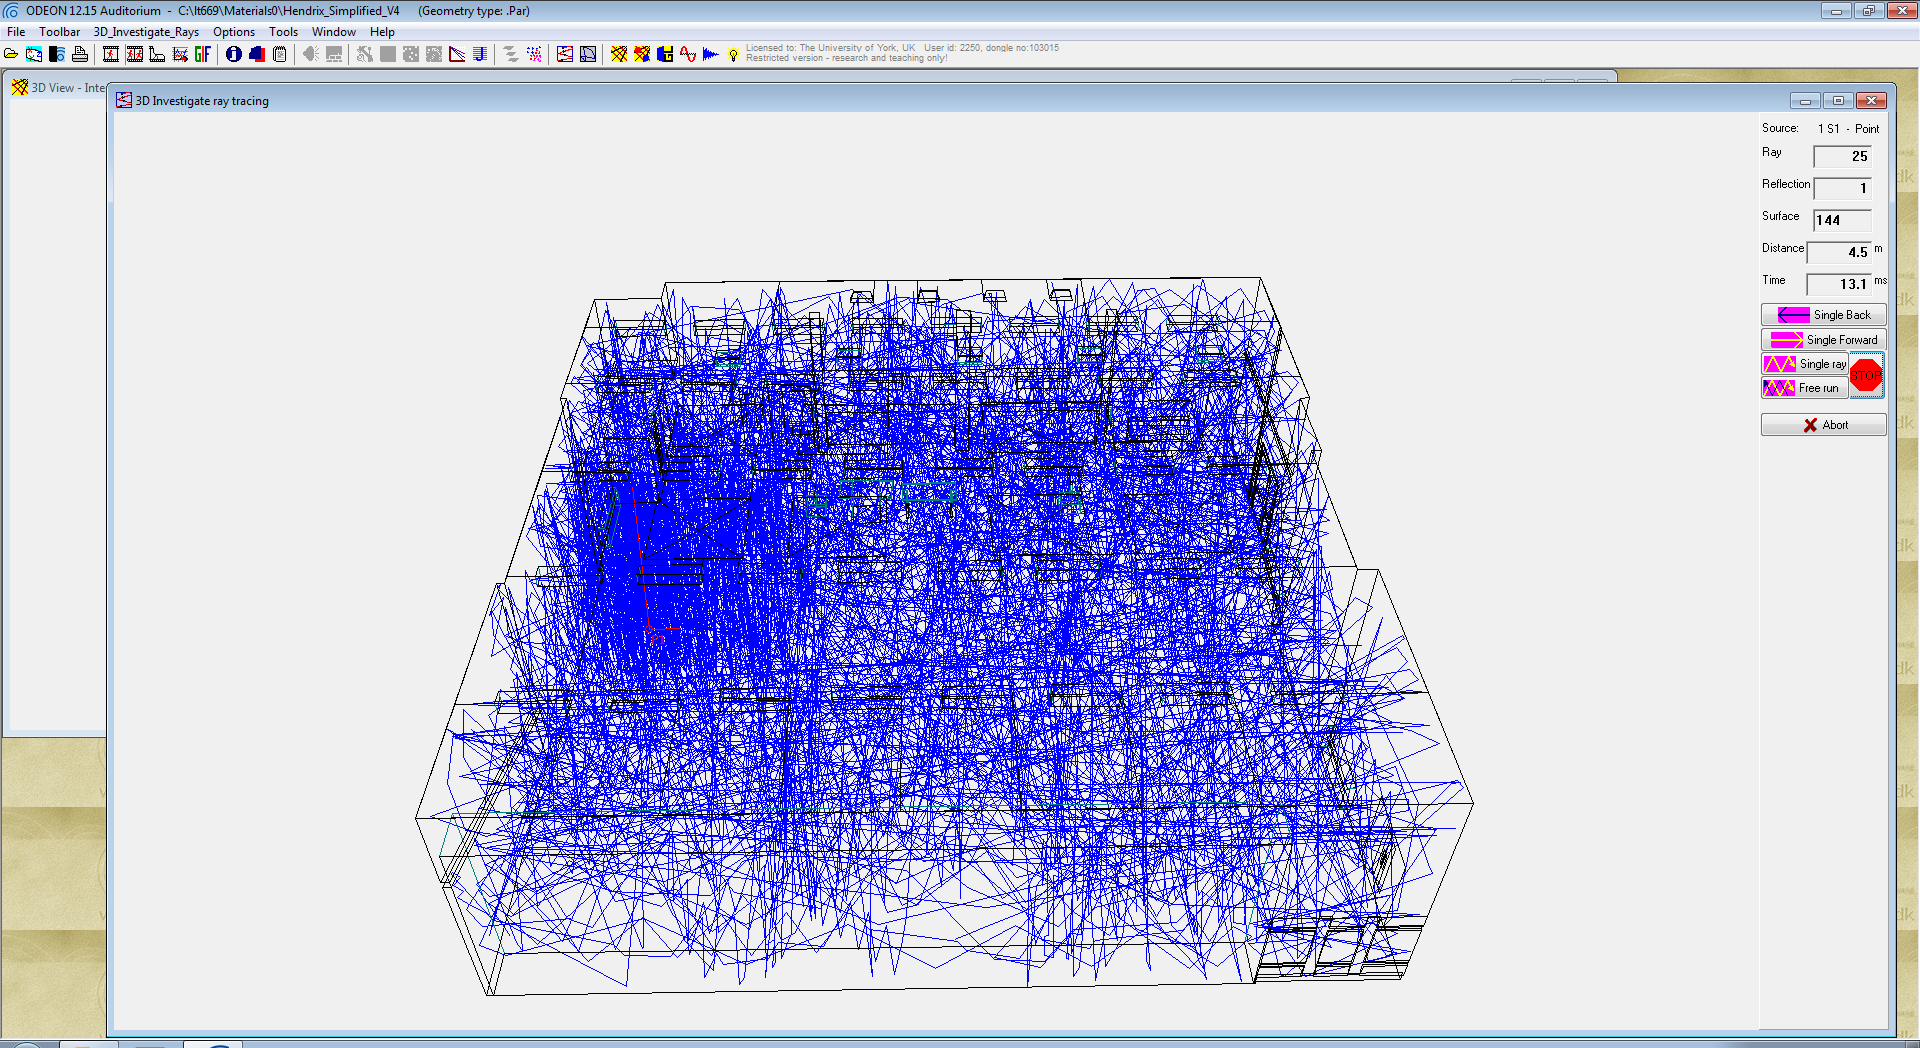
\includegraphics[scale = 0.3]{Sections/Implementation/Odeon/images/OdeonRays/waterTight2.PNG}}
			\caption{Hendrix Hall model undergoing a water tightness test in Odeon.}
			\label{watertight}
		\end{figure}

	\subsubsection{Material Selection}
	\label{odeon:materials}
		Surface materials greatly influence how sound reflects around a room, effecting reverberation time and the rate at which frequency bands are absorbed. It is therefore imperative to assign materials that closely match those within the real room in order to produce an accurate representation of the acoustic environment. For this, Odeon provides a list of common materials often found when constructing buildings.

		\paragraph{Initial Materials}

			Odeon's material list appears to be designed for the auralisation of structures with very basic interior. Due to a lack of choice, exact materials in the room could not be modelled accurately, however, the closest match to what was thought to be the true material were selected as an approximation. In some cases, appropriate replacement materials were not available, therefore new materials had to be added to the material list. This can be done by finding a materials absorption coefficients and selecting `\textbf{Edit an existing material}' where a new materials absorption coefficients can be entered and saved, as shown in figure~\ref{materialEdit}. Absorption coefficient values range from 0 - 1 (0\% - 100\%), indicating the percentage of attenuation applied to the selected frequency band upon a contact with the surface. Required materials for which an appropriate replacement could not be found in the material list are listed in table~\ref{materialTable}.

			\begin{table}[H]
			\begin{center}
				\begin{tabular}{r l}
					\textbf{Material} & \textbf{Surface applied to} \\ \hline
					Hard Plastic \cite{plastic} & Roof lights and projector covers \\
					Mineral fibre \cite{mineralFibre} & Ceiling Tiles \\
					Slate \footnotemark[1] \cite{Kovalchik} & Blackboard \\
				\end{tabular}
			\end{center}
			\caption{Table of materials for which absorption coefficients were sought and added to Odeon's material list.}
			\label{materialTable}
			\end{table}

			%-------------Footnote-------------%			
			\footnotetext[1]{The absorption coefficients provided were only available for the 125Hz to 4kHz octave bands, therefore absorption coefficients for the 63Hz and 8kHz octave bands were given a value of 0.1}

			%-------------Material Edit Image-------------%
			\begin{figure}[H]
				\centerline{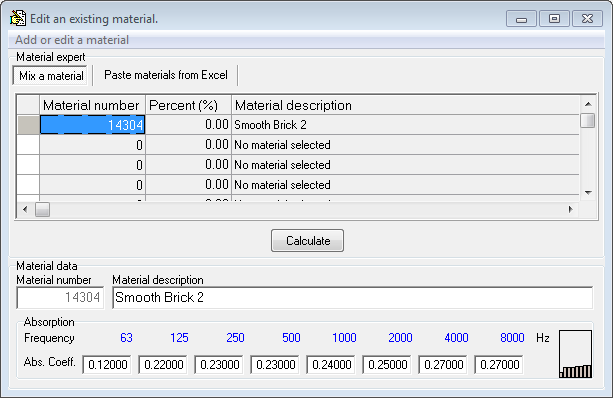
\includegraphics[scale = 0.9]{Sections/Implementation/Odeon/images/Absorption.PNG}}
				\caption{Absorption coefficient editing window in Odeon used to add unavailable materials.}
				\label{materialEdit}
			\end{figure}

		\paragraph{Surface Types}
			\label{surfaceTypes}

			For a number of surfaces it is appropriate to edit properties other than just their absorption coefficients. As explained in section \nameref{designRoom}, the roof hangings are constructed of four joint slanting surfaces. By changing the individual surface types from \textbf{`Normal'} to \textbf{`Fractional'}, Odeon avoids erroneously calculating diffraction due to each of the individual surfaces and treats them as a whole surface. For surfaces such as the contracted seating shown in figure~\ref{seating} where gaps are present in the overall structure, it was possible to model this as one solid object and to set a \textbf{transparency} value. A transparency value of 0 means the surface is a solid, whereas a value of 1 makes a surface totally transparent, allowing rays pass to straight through it. A transparency value of 0.3 was chosen as a reasonable estimate, the effects of which are shown in figure~\ref{transparency}, showing how a ray can pass through the front of the object, reflect around the inside and eventually reflect back out again.


				%-------------Seating Image-------------%
			\begin{figure}[h]
				\centerline{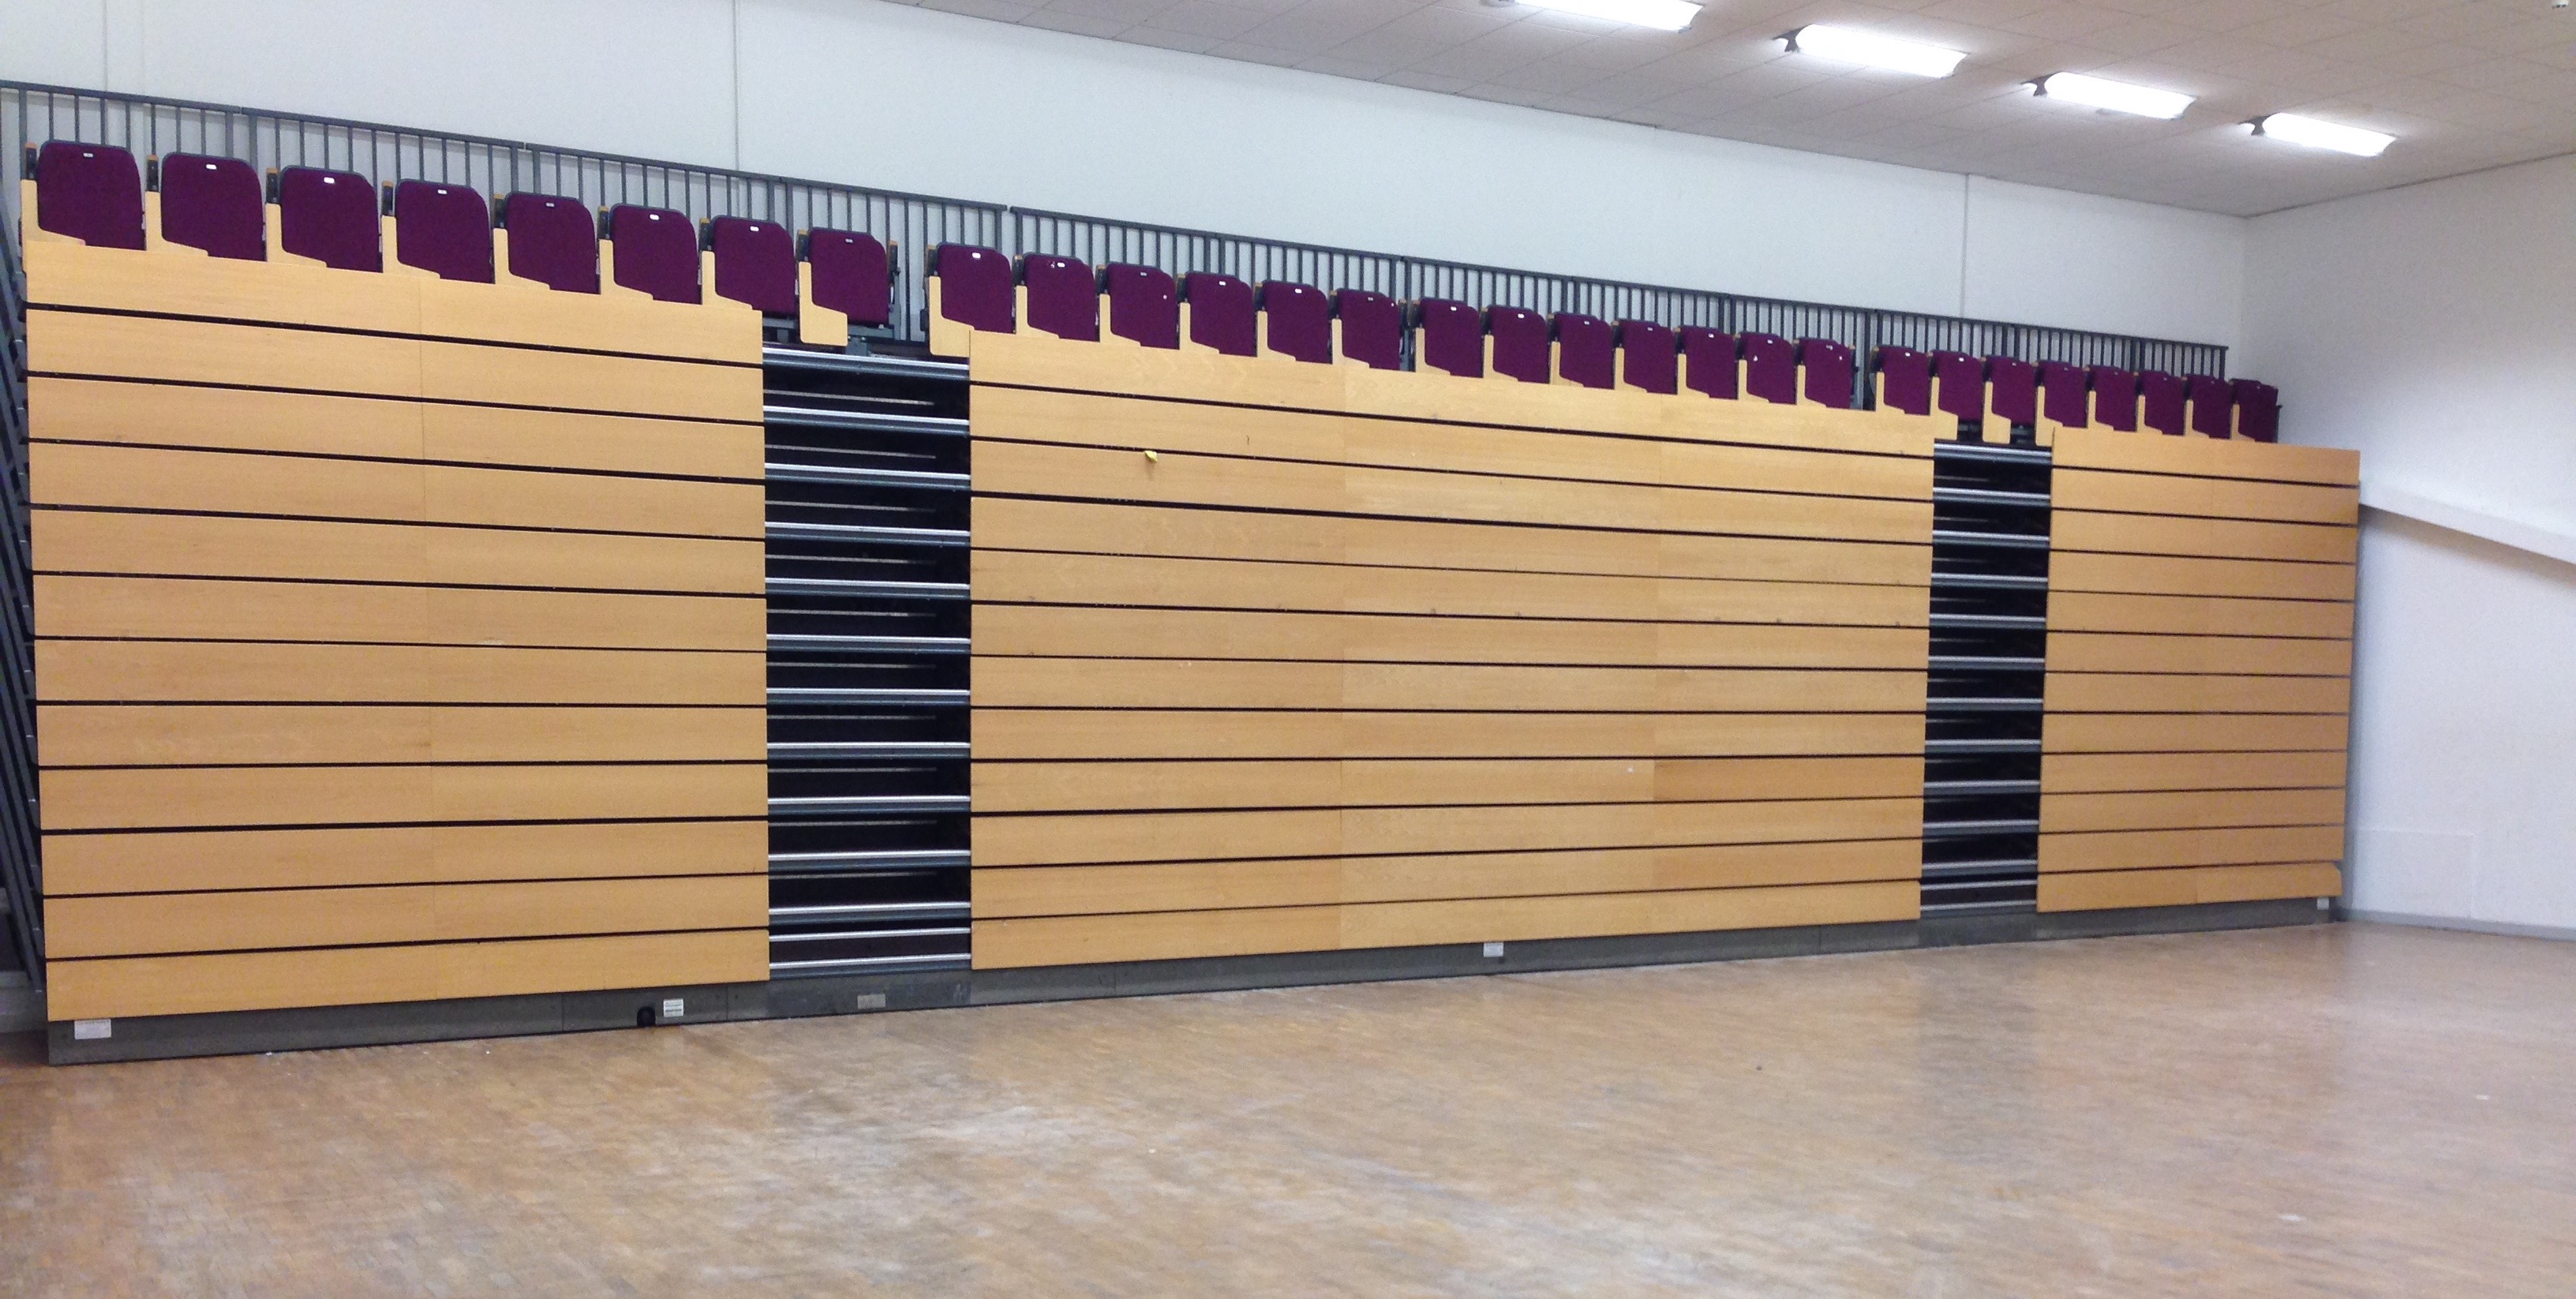
\includegraphics[scale = 0.12]{Sections/Implementation/Odeon/images/seating.jpg}}
				\caption{Contracted seating in Hendrix Hall showing gaps in the structure.}
				\label{seating}
			\end{figure}

			%-------------Transparency Image-------------%
			\begin{figure}[h]
				\center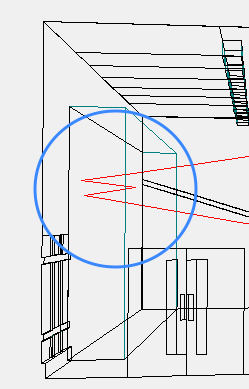
\includegraphics[scale = 0.7]{Sections/Implementation/Odeon/images/OdeonRays/transparencyEdit/singleRay2_edit3.PNG}
				\caption{Blue circle highlights a ray penetrating the modelled seating area, reflecting 3 times and escaping the seating area due to the transparency value set.}
				\label{transparency}
			\end{figure}

			As previously mentioned in section~\nameref{designRoom}, the lights were modelled as simple rectangles as opposed to the more complex objects made from a large number of surfaces with the intention of more accurately modelling the scattering effect (described in section~\nameref{background:scattering}) due to their shape by altering the objects \textbf{Scattering Coefficient}. Odeon provides a table of initial indicators for possible scattering coefficients, shown in figure~\ref{odeonTable} which can be used to select the scattering coefficient for a surface that fits a similar description to the one given. Given the vague descriptions, a scattering coefficient of 0.2 was selected for the lights.

			%-------------Scattering Coefficients table-------------%
			\begin{figure}[H]
				\centerline{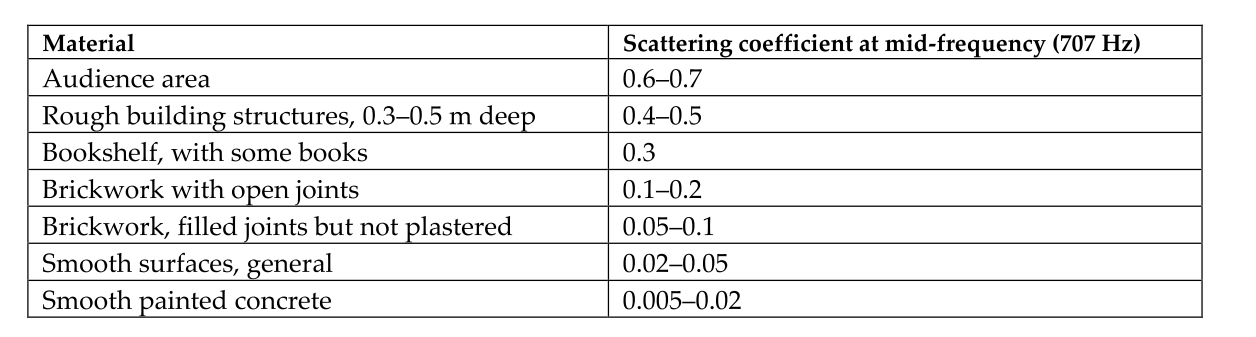
\includegraphics[scale = 0.3]{Sections/Implementation/Odeon/images/scatteringCoefficients.png}}
				\caption{A table provided in the Odeon Manual \cite{odeonManual} that can be used to set an approximate scattering coefficient for surfaces similar to those described.}
				\label{odeonTable}
			\end{figure}
		
		\paragraph{RIR Comparison}
			\label{rirComparison}

			Once the initial materials had been selected, the authenticity of the \ac{RIR}'s were checked by comparing their frequency content against that of a real measured \ac{RIR} from Hendrix Hall (see section~\nameref{realRIRs}). This was done by using Matlab to plot the spectrograms of the omni-directional W channel of both \ac{RIR}'s, as can be seen in figure~\ref{compareOriginal}. The spectrogram shows the high frequency content in the real \ac{RIR} attenuating in a smooth roll off fashion from 20kHz to about 8kHz starting from approximately 0.2 seconds in, whereas the full audible spectrum appears to attenuate almost evenly in the \ac{RIR} produced in Odeon.

			%-------------Original materials compare-------------%
			\begin{figure}[H]
				\centerline{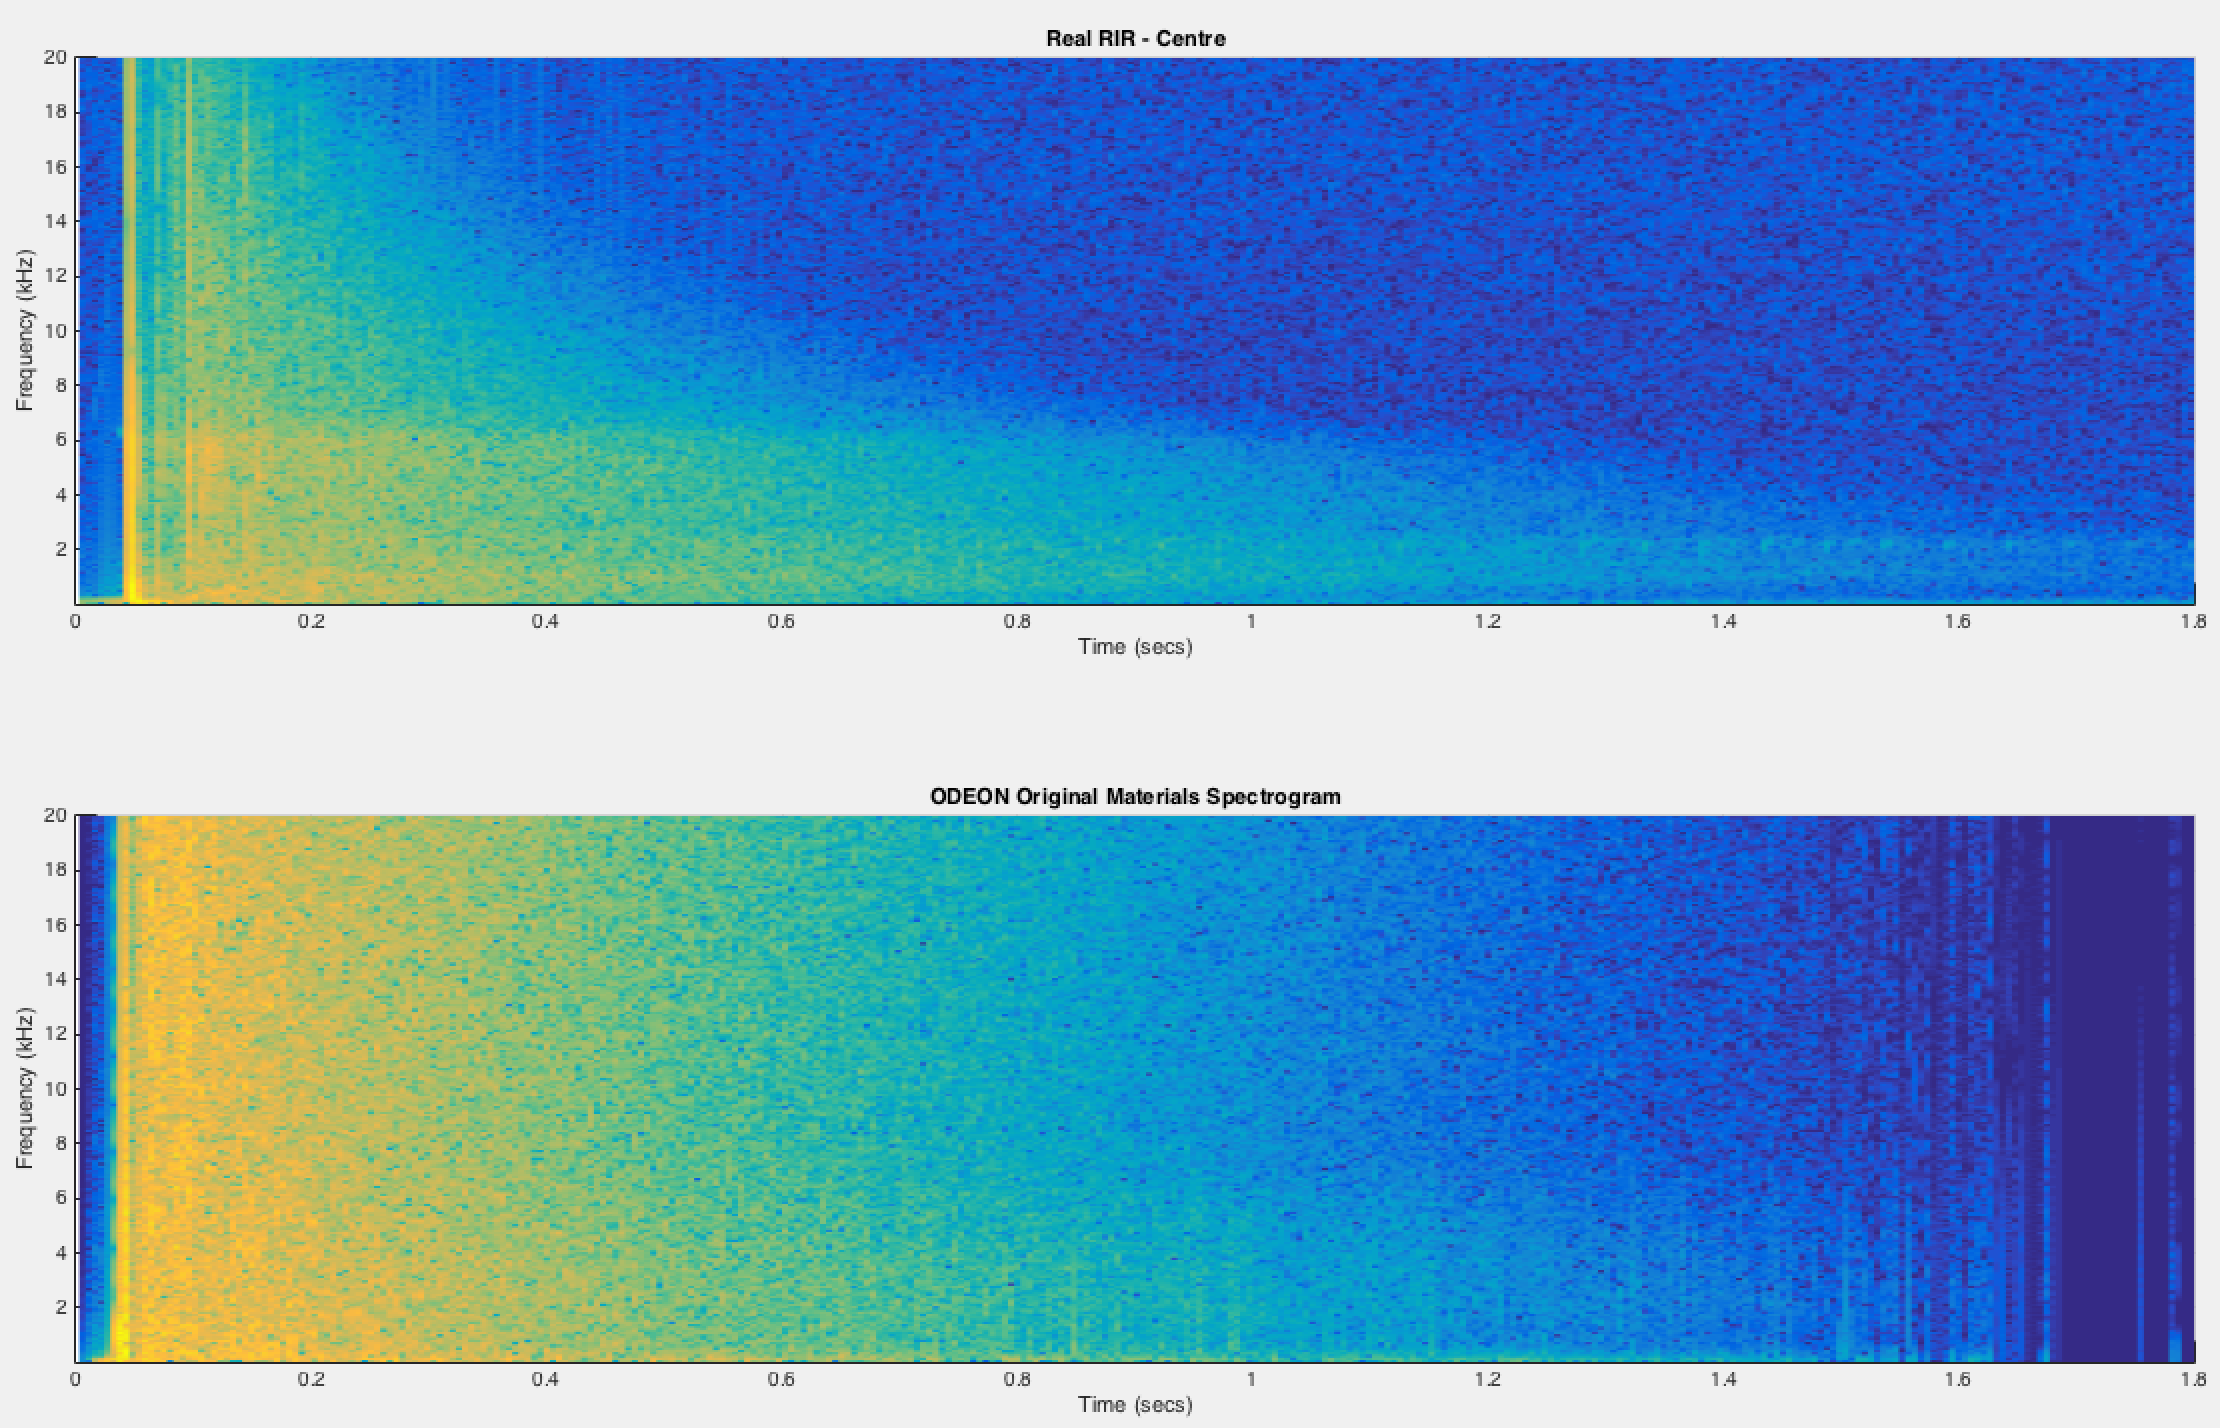
\includegraphics[scale = 0.3]{Sections/Implementation/Odeon/images/MaterialCompare/OriginalMaterials/original.png}}
				\caption{Spectrograms of real \ac{RIR} (top) against spectrogram of first rendered \ac{RIR} from Odeon.}
				\label{compareOriginal}
			\end{figure}

			 As the most obvious difference between the two is the difference in high frequency attenuation, large surfaces with low valued high frequency absorption coefficients, such as the walls and ceiling, were edited to absorb more of the high frequency content. Several iterations can be seen in figure~\ref{compareAll}, showing the spectrogram of the real \ac{RIR} and several iterations of the \ac{RIR}'s rendered from Odeon. The Spectrogram at the bottom is that of an \ac{RIR} produced in Odeon with the final material selections. The difference between the real RIR and the final Odeon \ac{RIR} can be seen more clearly in figure~\ref{compareNew}. This was done by adding 10\% onto the existing absorption coefficients for the 63Hz - 2000Hz octave bands, 20\% to the 4000Hz band and 30\% to the 8000Hz band. This also included editing the ceiling material coefficients by adding an extra 10\% to the 8000Hz octave band.

			Table~\ref{materialTable} contains a list of audio samples (can be found \href{http://lt669.github.io/pages/audioSamples.html}{here} or in file 1.4) indicating the edits made to the material list in order to produce each one, with their corresponding spectrogram graph name which can be found in figure~\ref{compareAll}.

			%-------------Audio Samples Table-------------%
			\begin{table}[h]
				\centering
				\begin{tabular}{|l | l | c | c | c |} 
					\hline
					\multirow{2}{*}{\textbf{Audio file}} & \multirow{2}{*}{\textbf{Graph Name}} & \multicolumn{3}{c|}{\textbf{Absorption Coefficient Edits}} \\ \cline{3-5}
					 & & \textbf{Material} & \textbf{Addition} & \textbf{Octave band} \\ \hline
					RealRIR.wav & Real RIR & \multicolumn{3}{c|}{NA}\\ \hline
					OdeonOriginal.wav & ODEON Original & \multicolumn{3}{c|}{NA}\\ \hline
					Odeon3RIR.wav & ODEON 3 & Ceiling (Mineral Fibre) & +10\% & 8kHz\\ \hline
					Odeon6RIR.wav & ODEON 6 & Walls (Solid Brick) & +10\% & All\\ \hline
					Odeon7RIR.wav & ODEON 7 & Walls (Solid Brick) & +10\% & 4kHz\\ 
					& & & +20\% & 8kHz \\
					& & Ceiling (Mineral Fibre) & +10\% & 8kHz\\ \hline
				\end{tabular}
				\caption{List of audio samples with corresponding spectrogram title in figure~\ref{compareAll} and the edits made for each one. (Only Odeon(3)(6)(7) audio sample are shown here as the other audio samples produced as a result of other material list iterations provided no relevant information).}
				\label{materialTable}
			\end{table}

			%Material selection conclusion
			By analysing figure~\ref{compareNew} it can be seen that it was possible to produce a much more fitting \ac{RIR} compared to the one produced using the original materials. By listening to the audio samples, it is clear that though the final Odeon RIR (Odeon7RIR.wav) is much more similar to the real \ac{RIR} (RealRIR.wav) than the one produced using the original surface materials (OdeonOriginal.wav) in terms of reverberation time, they still sound very different in terms of their frequency content, where the \ac{RIR}'s produced in Odeon lack what the author considers \textit{depth}. This is most likely due to the fact that the geometrical acoustic modelling methods used to produce the \ac{RIR} do not accurately reproduce the low-frequency content, the reasons for which were discussed in \nameref{Software:Odeon}. However, it can be said that the final Odeon \ac{RIR} sounds much more similar to the real one than the other three \ac{RIR}'s produced using earlier iterations of the material list.

			%-------------All materials compare-------------%
			\begin{figure}[H]
				\centerline{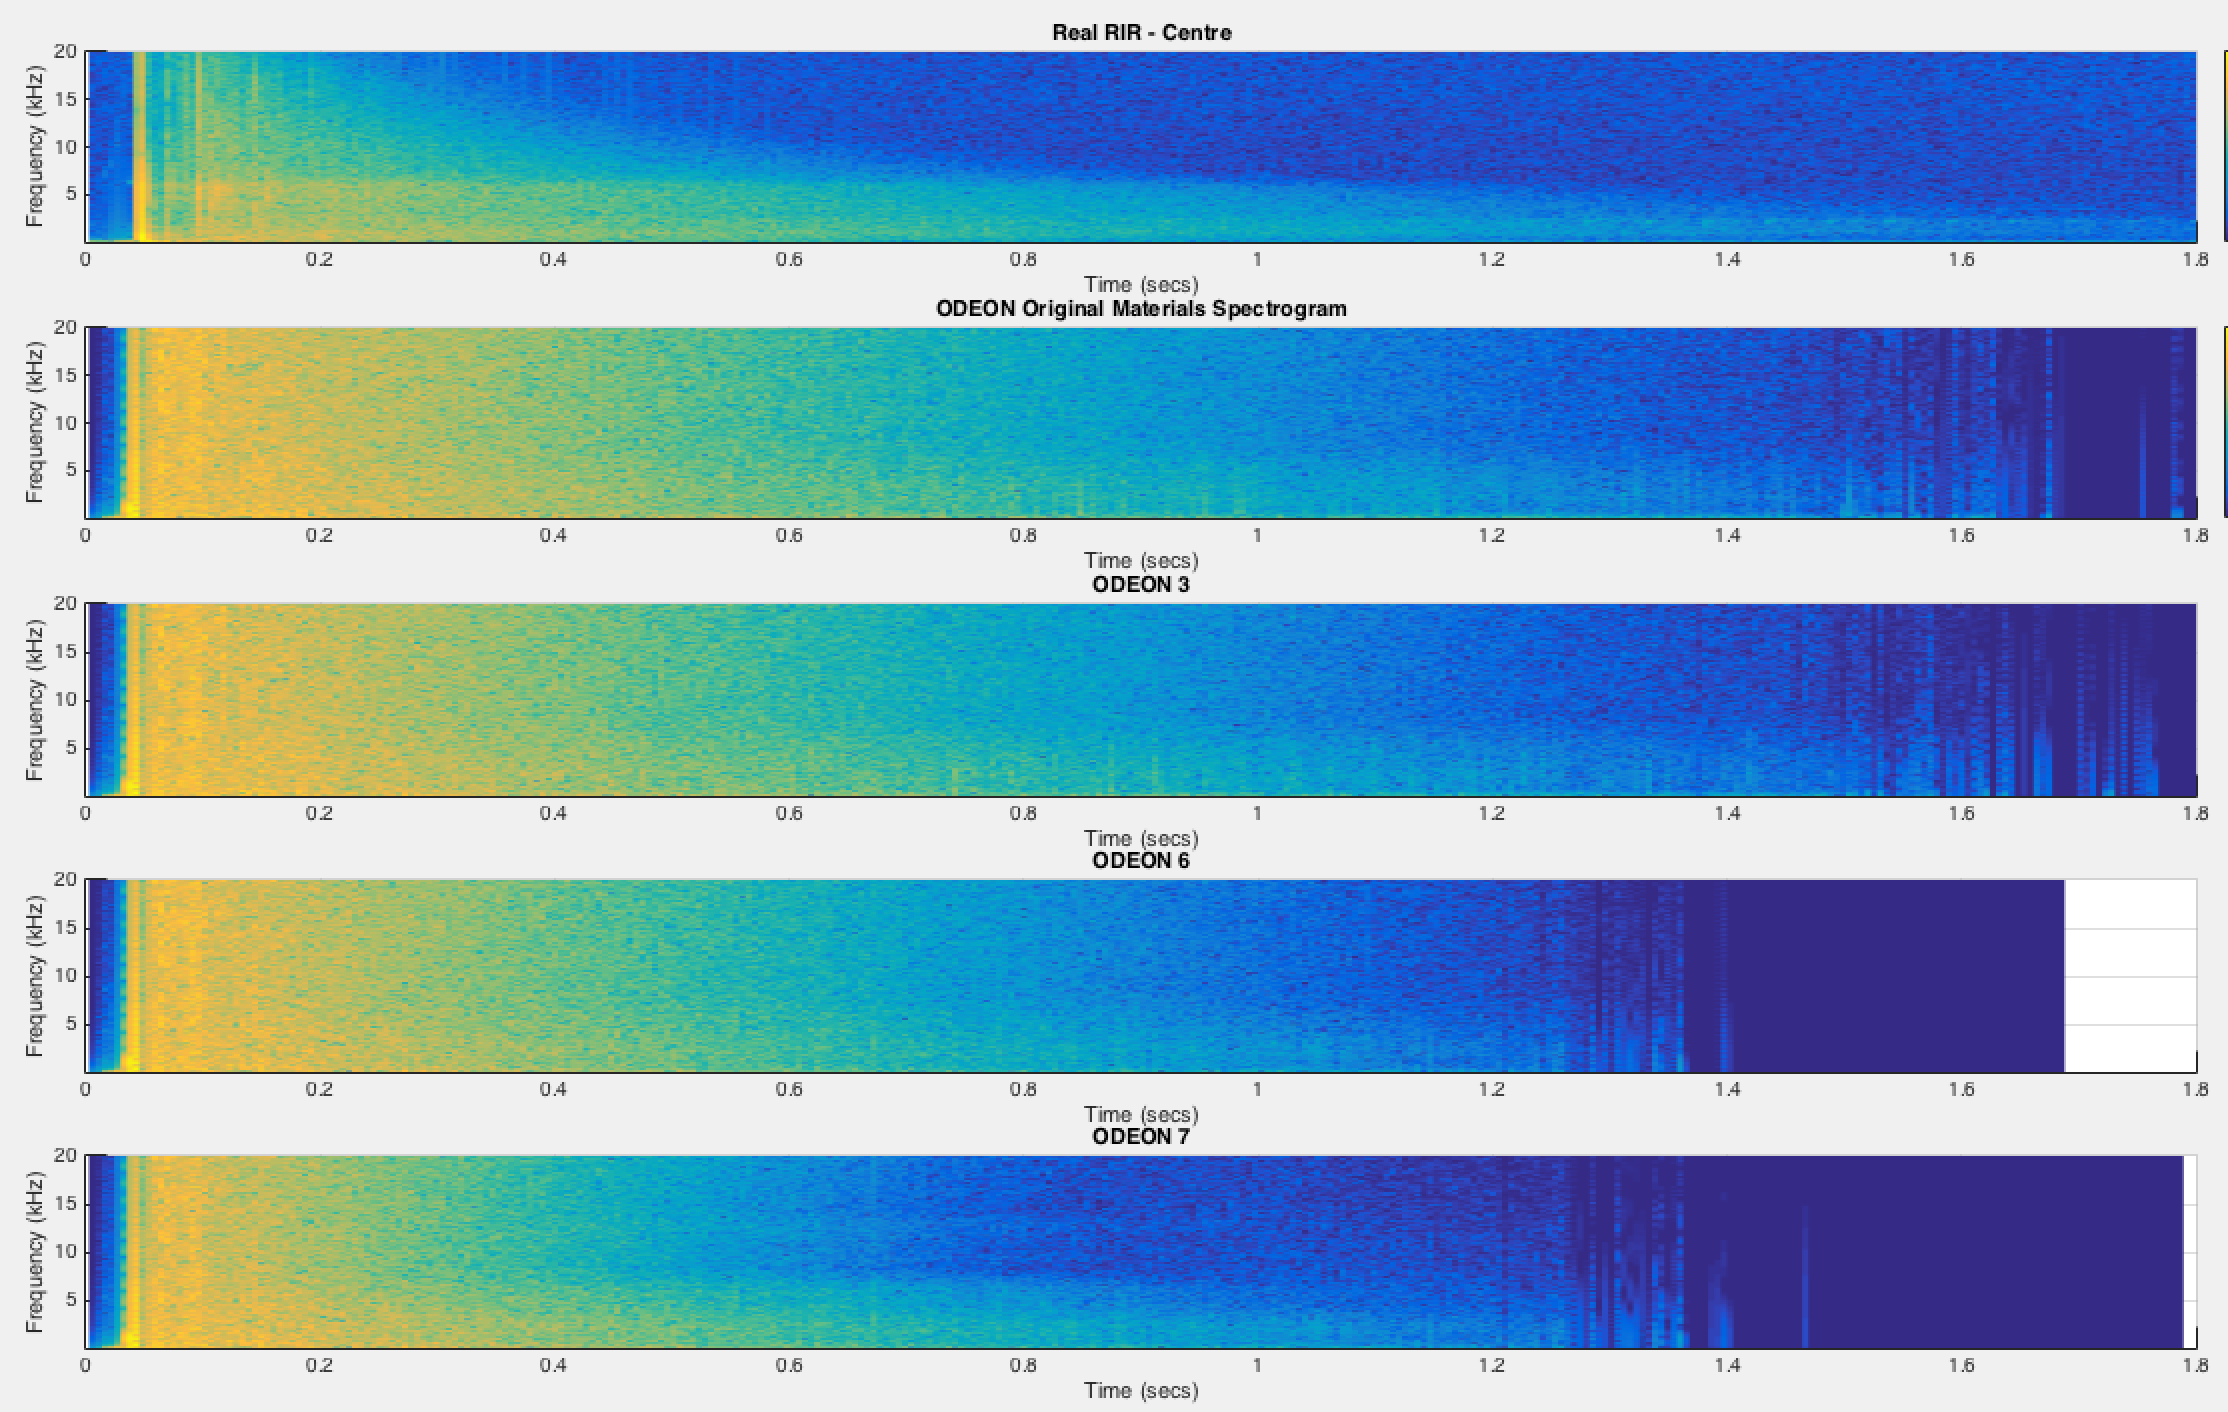
\includegraphics[scale = 0.45]{Sections/Implementation/Odeon/images/MaterialCompare/OriginalMaterials/all.png}}
				\caption{Spectrogram of real \ac{RIR} (top) against the spectrograms of several rendered \ac{RIR} from Odeon with different material absorption coefficients where ODEON (bottom) shows the final \ac{RIR} used. Spectrogram titles and corresponding material edits can be found in table~\ref{materialTable}}
				\label{compareAll}
			\end{figure}

			%-------------New materials compare-------------%
			\begin{figure}[H]
				\centerline{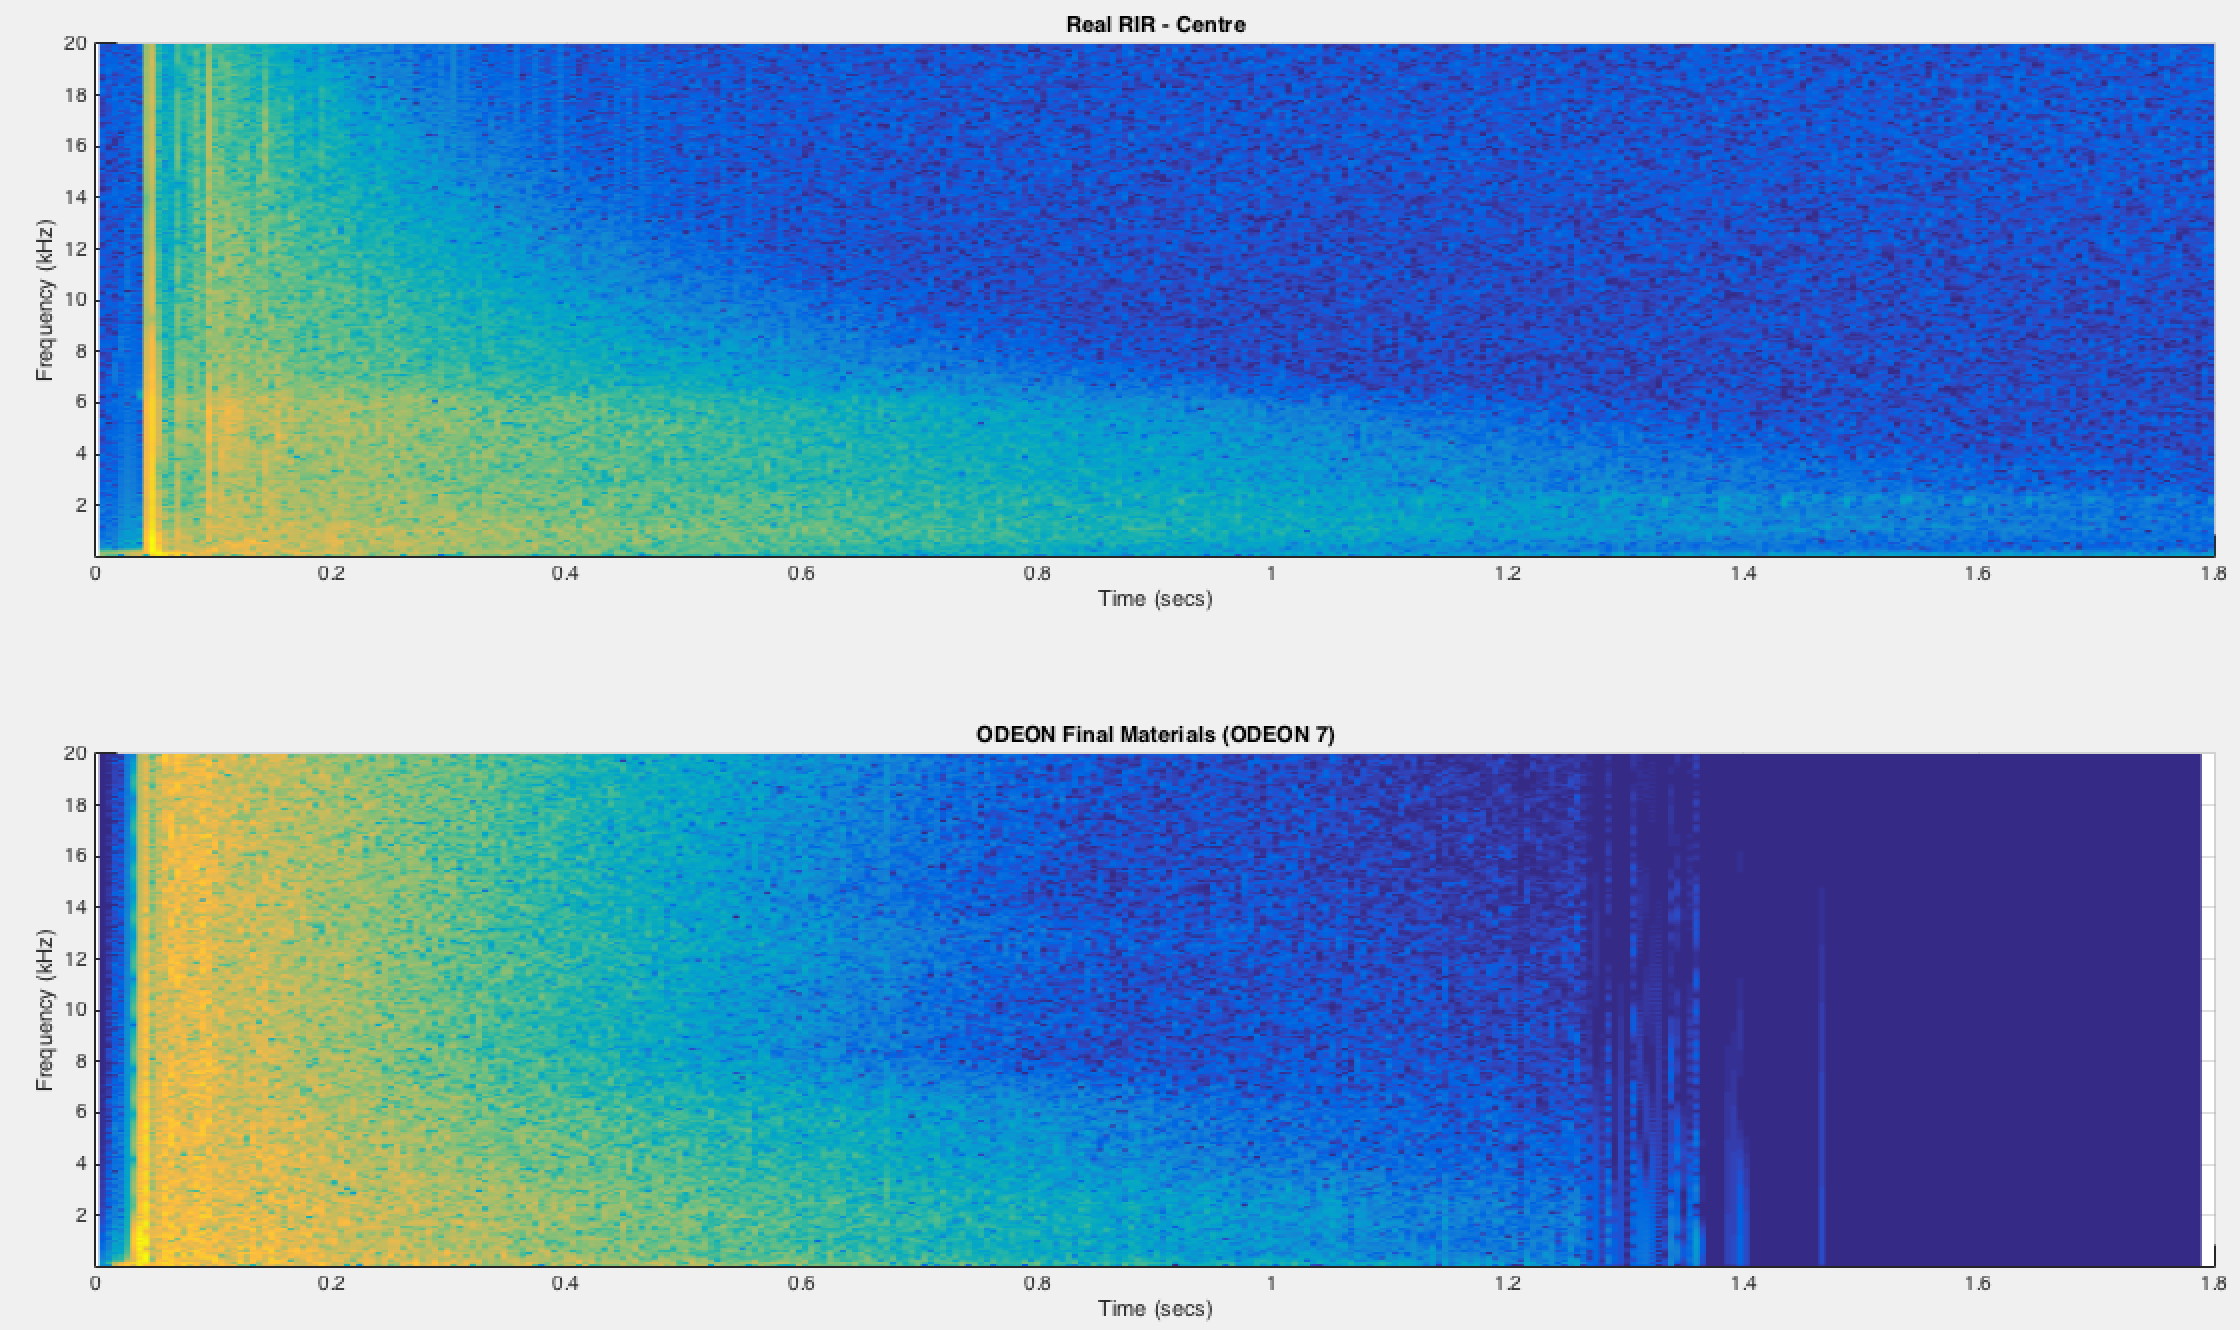
\includegraphics[scale = 0.4]{Sections/Implementation/Odeon/images/MaterialCompare/OriginalMaterials/new.png}}
				\caption{Spectrograms of real \ac{RIR} (top) against Odeon \ac{RIR} from Odeon with final material absorption coefficients showing a more convincing replica of the real \ac{RIR} by editing the rooms material absorption coefficients.}
				\label{compareNew}
			\end{figure}

			The full material list is available in \href{http://lt669.github.io/pages/Material_List_Final.htm}{Material\_List\_V2.xlsx}, showing which materials are applied to each surface within the Odeon model, as well as a list of absorption coefficients iterations that were applied to the brick walls and ceiling can be found in \href{http://lt669.github.io/pages/Absorption%20Coefficients.htm}{Absorption\_Coefficients.xlsx}. Both can also be found in file 4.3.

			%Mention incorrect RIRs
			It was later discovered (see section~\nameref{odeonError}) that the \ac{RIR}'s used to decide the final materials were incorrect, a result of which caused them to be much louder than they should have been. To ensure that the final surface materials that were selected when using the incorrect \ac{RIR}'s were still appropriate for the new, quieter ones, two new \ac{RIR}'s were rendered using both the original materials and the final materials. Both were plotted to compare against the same real \ac{RIR} used before, the results of which are shown in figure~\ref{compareCorrect}. As the new Odeon \ac{RIR}'s were so much quieter, the real \ac{RIR} was reduced in level to match those produced by Odeon. As it can be seen, the final materials used in the room model reduce the length of the reverb and attenuate high frequencies quicker than when the room model contained the original materials as they had shown previously.  

			%-------------Correct RIR materials compare-------------%
			\begin{figure}[H]
				\centerline{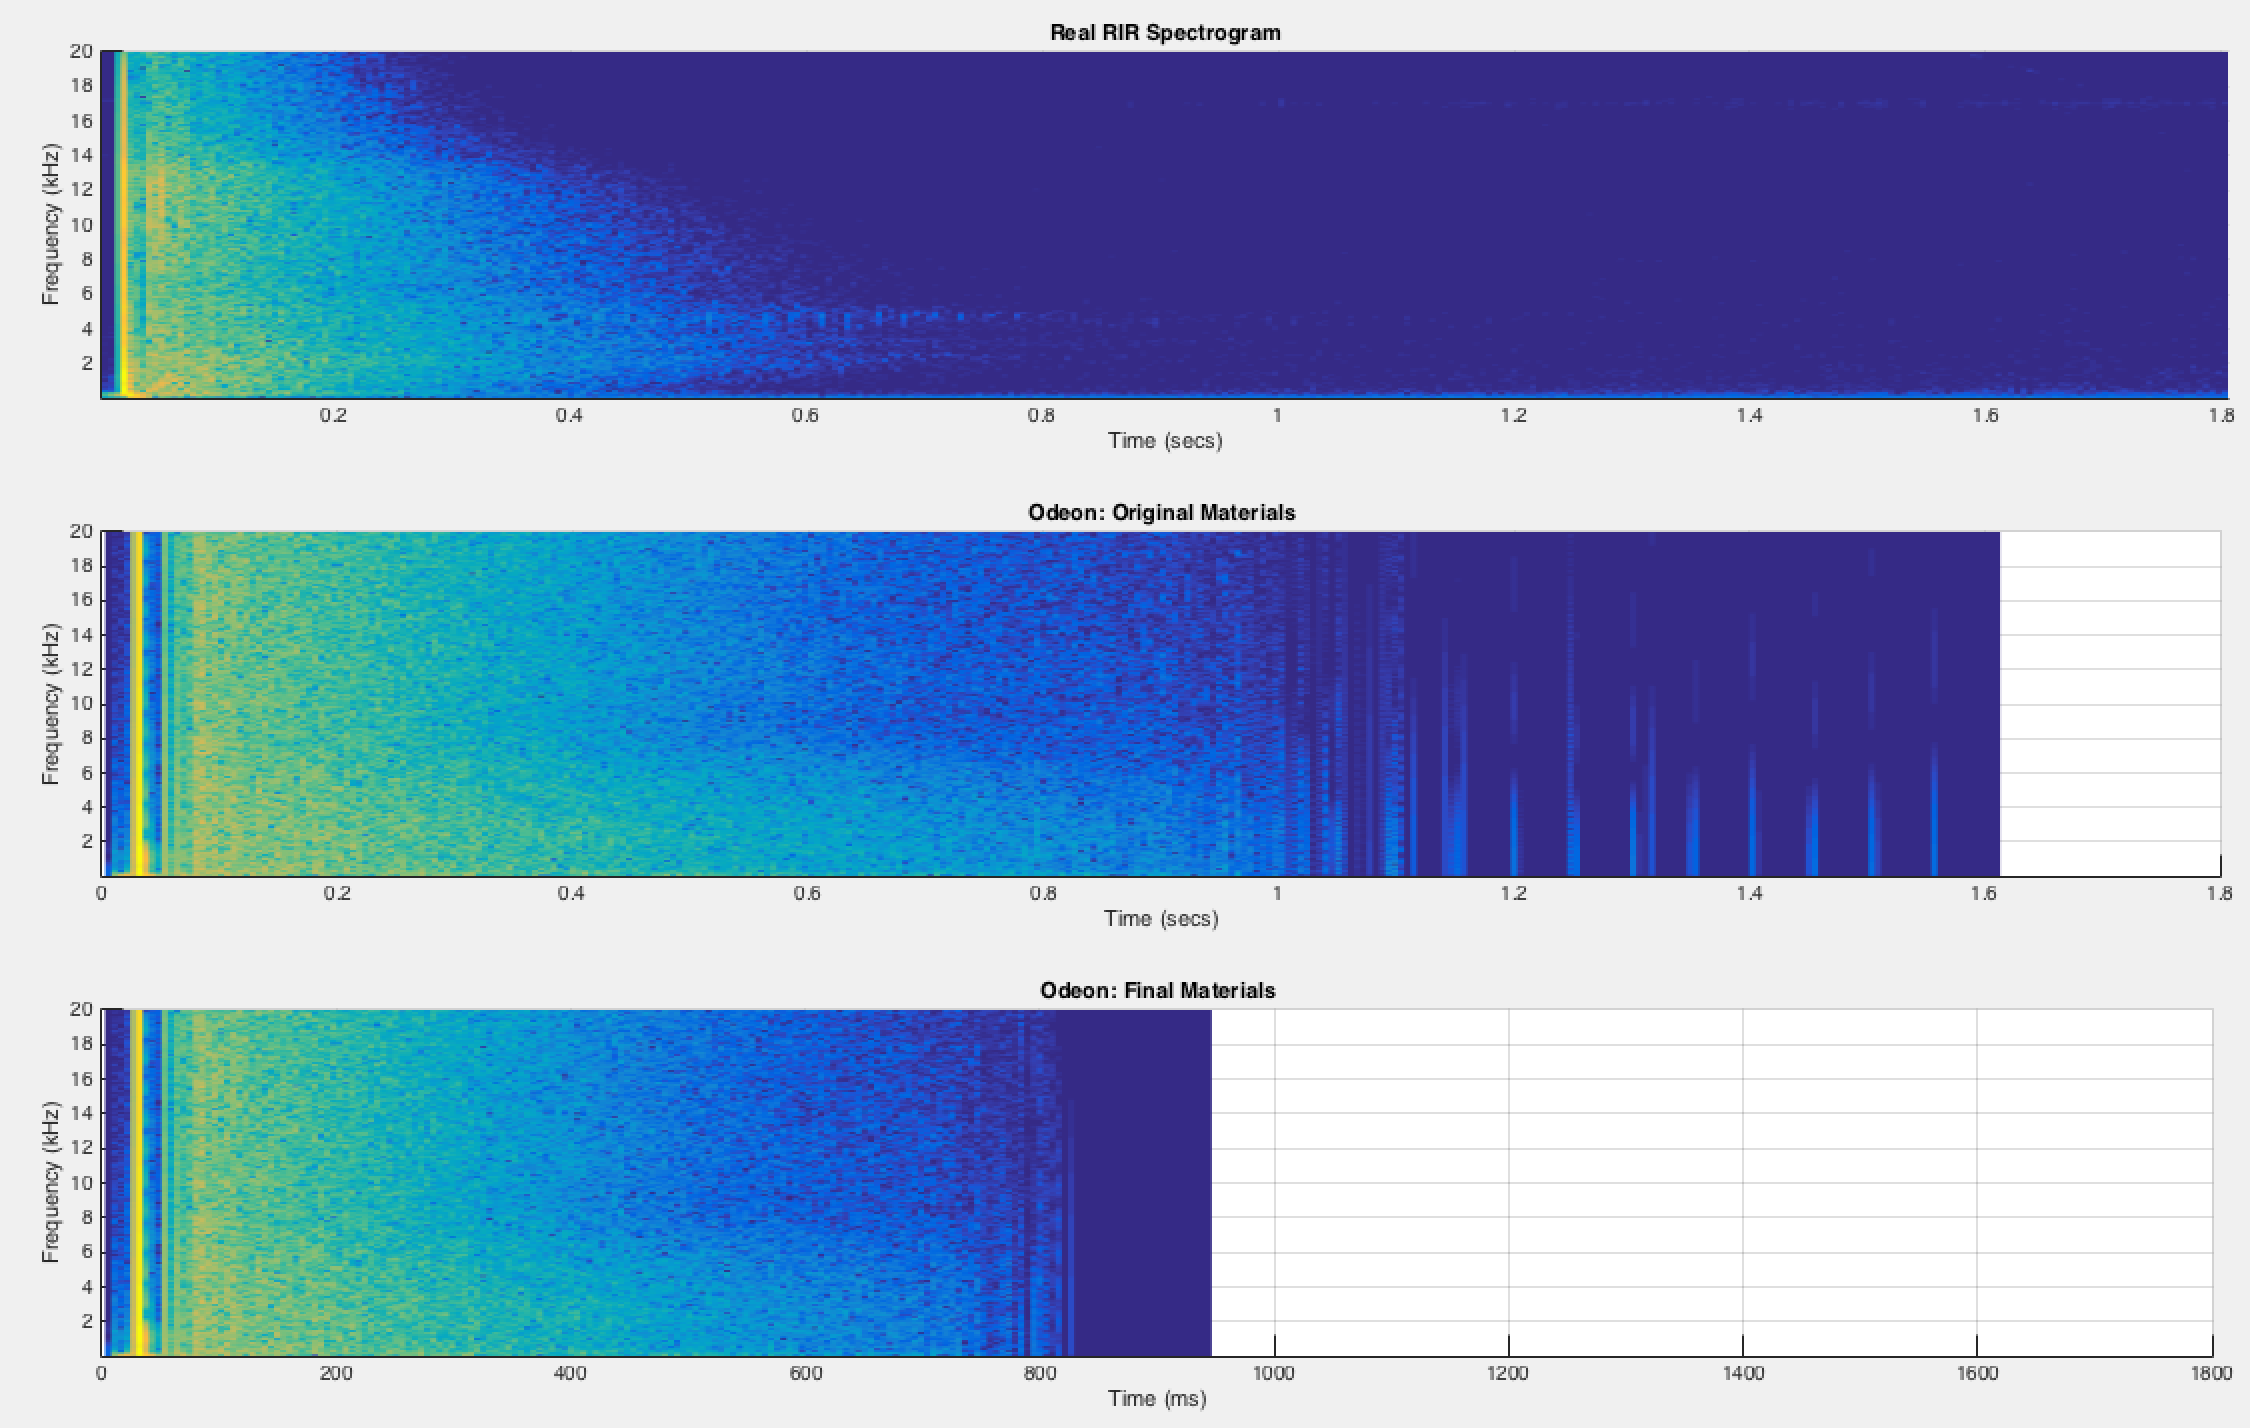
\includegraphics[scale = 0.4]{Sections/Implementation/Odeon/images/MaterialCompare/NewMaterials/newOdeonComparison.png}}
				\caption{Spectrograms of correct Odeon \ac{RIR}'s with original materials (top) and final materials (centre) to compare against real RIR that has been level calibrated (bottom).}
				\label{compareCorrect}
			\end{figure}

		\subsubsection{Odeon Output Settings}
			\paragraph{Ray Settings}

				%Other settings
				Odeon provides the following options for \ac{RIR} rendering:

				\textbf{Astop} - The maximum possible attenuation of each octave band.

				\textbf{Apass} - Ripple of octave band filters in dB.

				\textbf{Band overlap} - 100\% overlap gives a smooth transition between the FIR octave band filters as they are not completely rectangular.

				\textbf{Maximum reflection order} - Maximum allowed is 2000 as is the default. This means a ray can only reflect around a room 2000 times before the simulation is stopped. This prevents trapped rays from prolonging the impulse response if it never reaches the receiver.

				\textbf{Late Rays} - These are emitted from the source and reflected according to the \ac{VBS} (described in section~\nameref{background:scattering}) taking into account scattering due to surface size and roughness.

				\textbf{Transition Order} - As explained in section~\nameref{Software:Odeon}, a \ac{TO} can be set to determine the number of early rays sent out to find a number of wall combinations for reflections using the \ac{ISM}. After this number of rays has been reached, the ray-tracing method is used.

				All settings apart from \ac{LR's} and \ac{TO} are left at their default values as they are sufficient for accuracy and prevent the increase of computation time which will be needed given the large number of RIRs required for free movement.

				%TO and Late rays
				Odeon suggests two possible modes, \textbf{Engineer} and \textbf{Precision} which both suggest using a different number of \ac{LR's} which are 1285 and 20560 respectively. As both the \ac{TO} and \ac{LR's} value increase both the accuracy and computation time of the \ac{RIR}'s, different combinations of the values were tried and \ac{RIR}'s were rendered for comparison. Figure~\ref{odeonSettingsRIR} shows plots of the rendered \ac{RIR}'s with the name indicating the \ac{TO} and \ac{LR's} value. For example, `TO\_2\_LR\_1285' indicates the sample was produced where \ac{TO} = 2 and \ac{LR's} = 1285. Table~\ref{odeonSettingsTable} can be used to clarify the settings used for each \ac{RIR} in figure~\ref{odeonSettingsRIR} and indicates which audio sample can be listened to. For consistency, all \ac{RIR}'s were taken from the centre of the modelled room.

				\begin{table}
				\begin{center}
					\begin{tabular}{|l | c | l | l|}
					\hline
					\textbf{Audio Sample} & \textbf{\ac{TO}} & \textbf{\ac{LR's}} & \textbf{Graph Name}\\ \hline
					TO\_2\_LR\_1285.wav & 2 & 1285 & TO\_2\_LR\_1285 \\
					TO\_2\_LR\_20560.wav & 2 & 20560 & TO\_2\_LR\_20560 \\
					TO\_4\_LR\_1285.wav & 4 & 1285 & TO\_4\_LR\_1285\\
					TO\_4\_LR\_20560.wav & 4 & 20560 & TO\_4\_LR\_20560 \\ \hline
					\end{tabular}
				\end{center}
				\caption{Table of audio samples with the corresponding settings information and graph name. Samples can be listened to \href{http://lt669.github.io/pages/audioSamples.html}{here} or in file 1.3}
				\label{odeonSettingsTable}
				\end{table}


			%-------------TO and LR value image-------------%
			\begin{figure}[h]
				\centerline{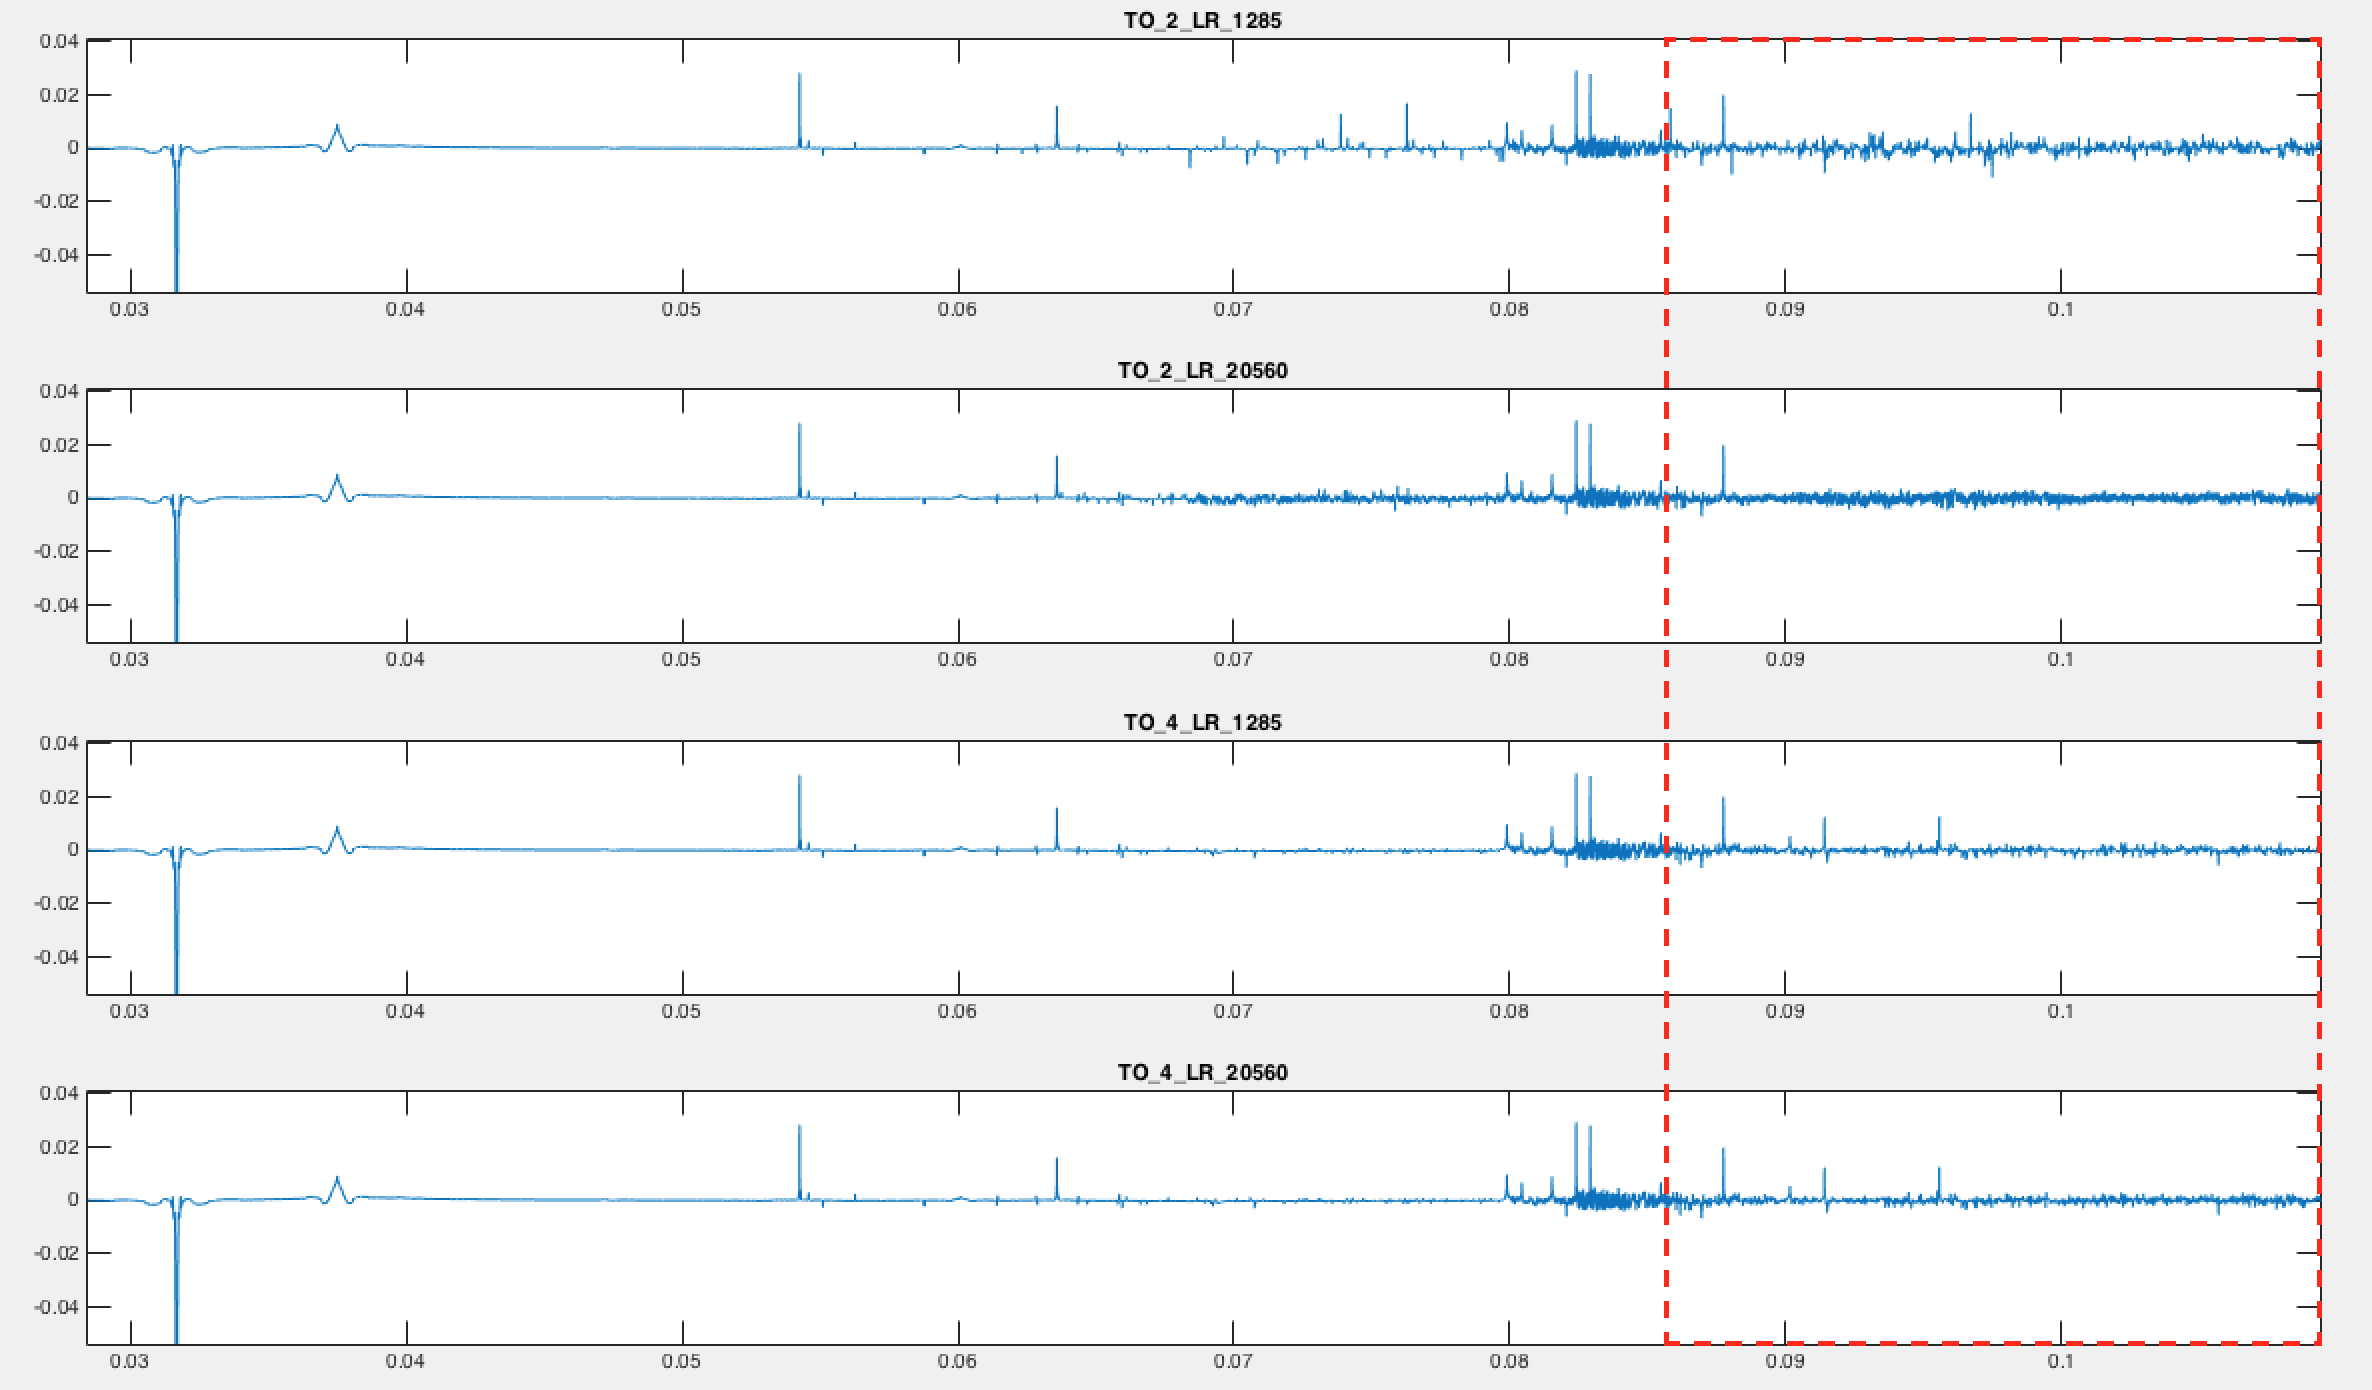
\includegraphics[scale = 0.35]{Sections/Implementation/Odeon/images/OdeonSettings/settingsFigure_edit.png}}
				\caption{\ac{RIR}'s rendered using different \ac{TO} and late ray values}
				\label{odeonSettingsRIR}
			\end{figure}
				%-------------TO and LR value Zoomed image-------------%
			\begin{figure}[h]
				\centerline{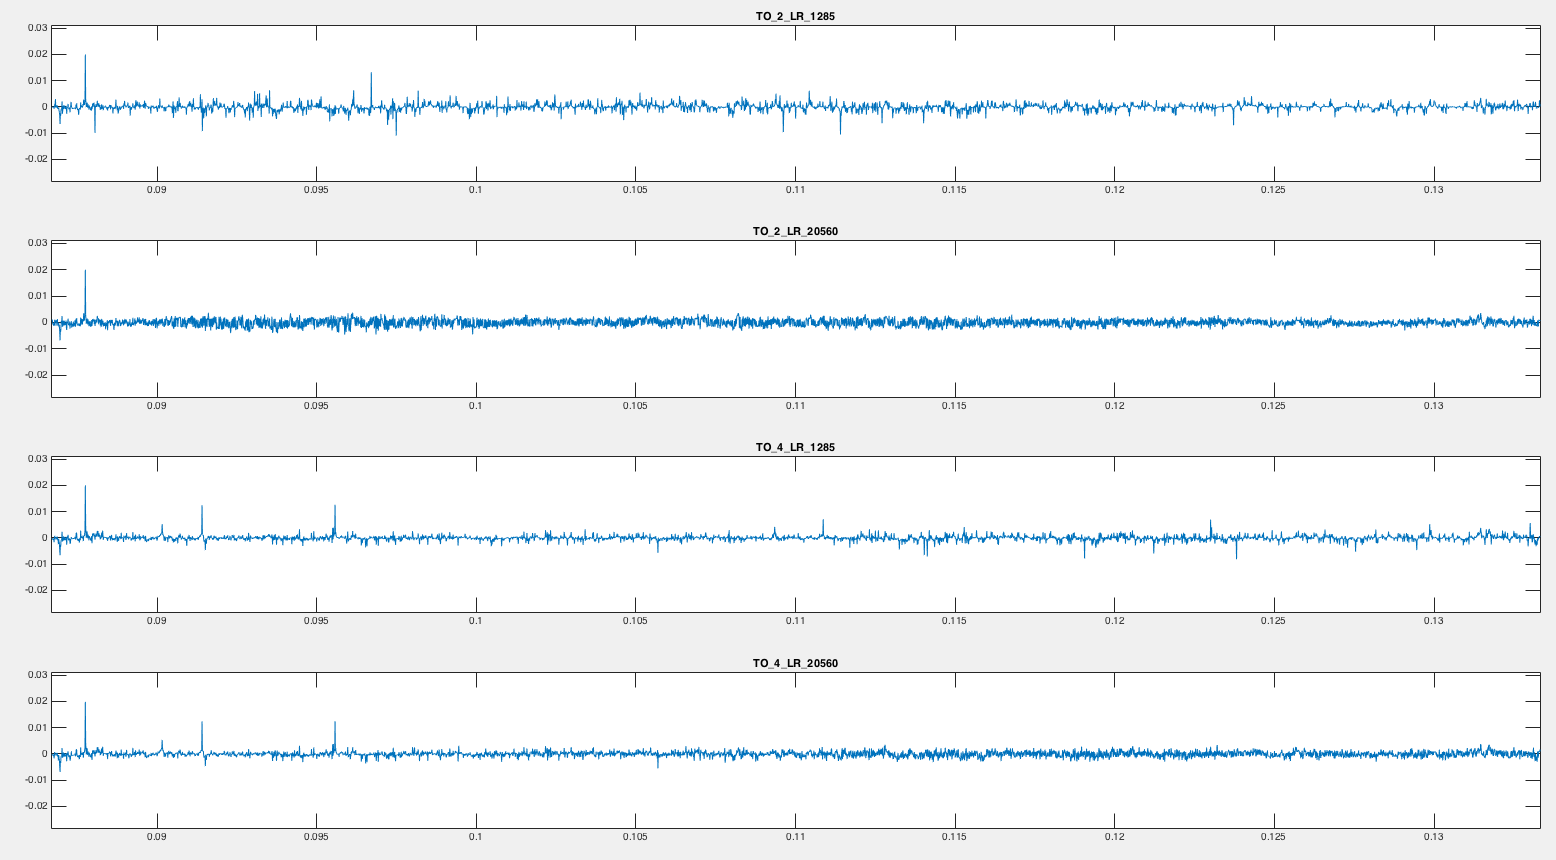
\includegraphics[scale = 0.33]{Sections/Implementation/Odeon/images/OdeonSettings/settingsFigureZoomed.png}}
				\caption{Zoomed in section indicated by the red dashed line in figure~\ref{odeonSettingsRIR}}
				\label{odeonSettingsRIRZoomed}
			\end{figure}

				%-------------TO Zoomed image-------------%
			\begin{figure}[h]
				\centerline{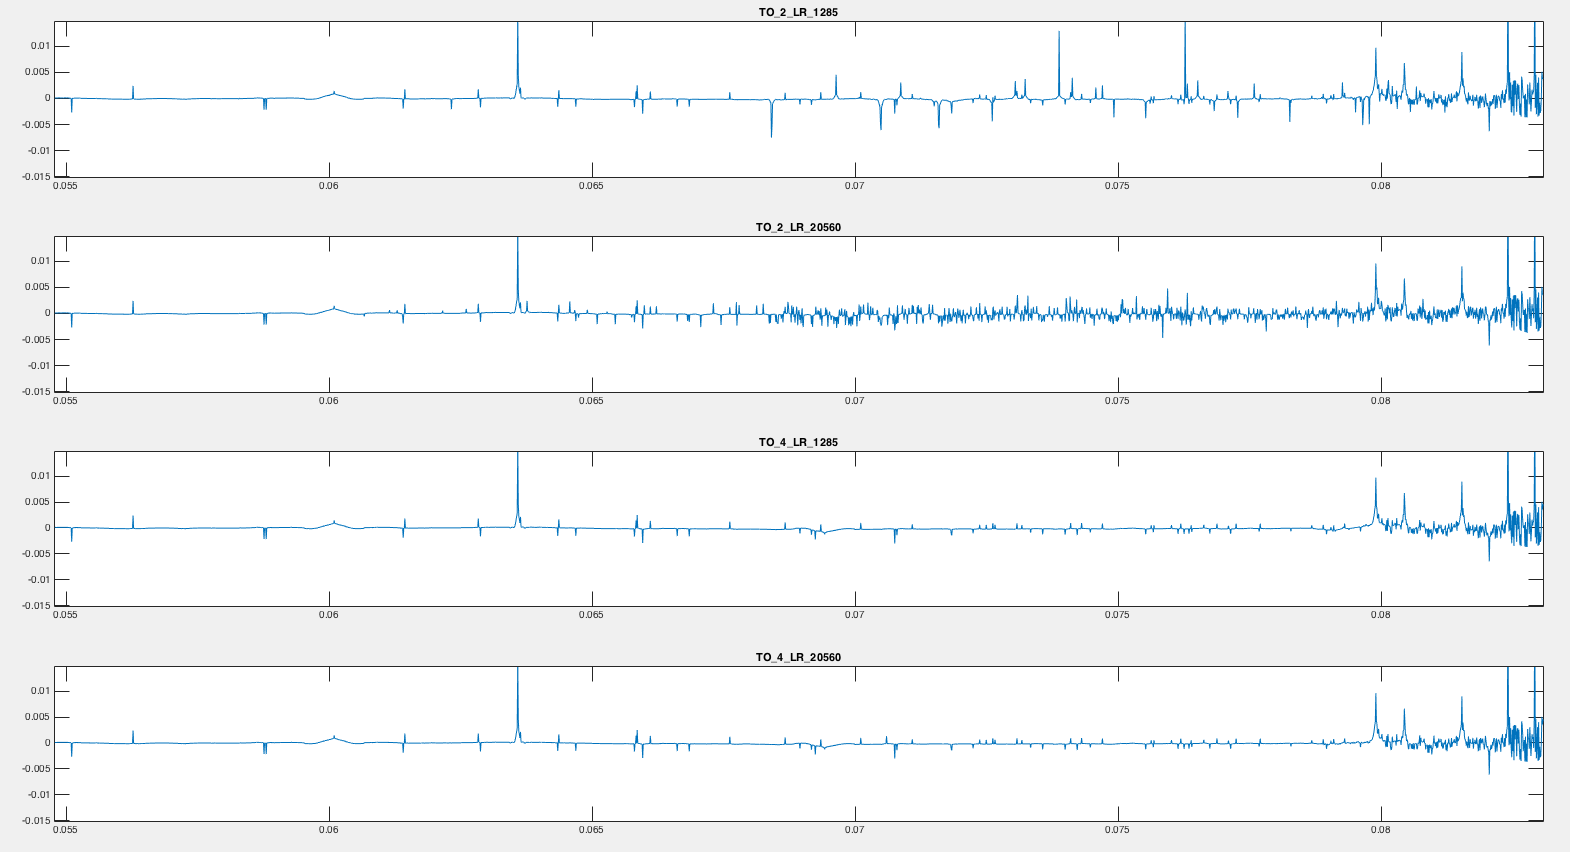
\includegraphics[scale = 0.35]{Sections/Implementation/Odeon/images/OdeonSettings/settingsFigure_TOZoom.png}}
				\caption{Zoomed in section showing the effects of using a high \ac{TO} value}
				\label{odeonSettings_TOZoomed}
			\end{figure}

				Through aural analysis, it can be heard that the number of \ac{LR's} used has an audible impact, where a lower \ac{LR's} value produces an \ac{RIR} that sounds \textit{grainy}. This can be seen in figure~\ref{odeonSettingsRIRZoomed}, which is zoomed in on the section highlighted in red in figure~\ref{odeonSettingsRIR} showing the \ac{RIR}'s from approximately 0.085s, where the difference caused by the different setting combinations can be seen. The two \ac{RIR}'s with a high \ac{LR's} value (2nd and 4th plot) show more densely packed reflections due to the fact that more rays are used. This produces a `smoother' more natural sounding reverb tail.

				%Figure~\ref{odeonSettings_TOZoomed} shows the same \ac{RIR}'s from the start of the plots. It is here that the effects of the different \ac{TO} values can be seen. The two plots showing the \ac{RIR}'s with a \ac{TO} of 2 (1st and 2nd plots) show more random peaks reflections than the \ac{RIR}'s that used a \ac{TO} of 4. This is because it is at this point that the ray-tracing method has been used, whereas the bottom two plots with a \ac{TO} of 4 show less random reflections as the \ac{ISM} will still be in use, thus peaks due to random ray reflections do not occur. Though the difference in using a \ac{TO} of 2 or 4 can be seen, is not audible.

				Figure~\ref{odeonSettings_TOZoomed} shows the same \ac{RIR}'s from the start of the plots. For the \ac{RIR}'s produced with a \ac{TO} value of 2 (1st and 2nd plots), it can be seen that there are a lot more randomly occurring peaks than in the \ac{RIR}'s with a \ac{TO} value of 4. It is assumed that this is caused by the fact that the ray-tracing method is used much earlier on in the top two \ac{RIR} plots, thus the randomly reflected rays cause more randomly occurring peaks. Though the difference in using a \ac{TO} of 2 or 4 can be seen, it is not audible by listening to the \ac{RIR} audio samples.

				The time difference taken to render the \ac{RIR}'s is also an important factor when choosing which of these settings to use. Given the potentially large number of \ac{RIR}'s required, a slightly more accurate output may result in a much greater calculation time. Odeon uses information gathered when previously rendering \ac{RIR}'s to speed up calculations for other \ac{RIR}'s being rendered in the same room, however there initial time taken to calculate each of the \ac{RIR}'s was noted and compared for reference.

				Initially it was found that increasing the \ac{TO} value from 2 to 4 increased the time taken to render by approximately 20 seconds, at which point it was decided that a \ac{TO} value of 2 would be used, given that it made no perceptual difference. However, much later it was realised that inaccurate calculation times may have been given due to the fact the project was being stored on the University network, thus adding variable delay times. The project was later stored on a local C drive, eliminating any network speed issues and inconsistencies. After doing so, the difference in \ac{TO} values made almost no difference to the calculation times. In hindsight, a higher \ac{TO} value could have been used to produce more accurate \ac{RIR}'s.

				It was found that the \ac{LR's} value made quite a difference to the calculation time:

				\begin{center}
					\begin{tabular}{c c c}
					\textbf{Transition Order} & \textbf{Late Ray Value} & \textbf{Calculation Time (s)} \\ \hline
					2 & 1285 & 11 \\
					2 & 20560 & 28 \\
					4 & 1285 & 11 \\
					4 & 20560 & 28 \\
					\end{tabular}
				\end{center}

				Despite the increase in calculation time by 17 seconds, the inaccuracy of \ac{RIR}'s produced when using the lower \ac{LR's} makes using the higher value justifiable.

				%B-Format setting
				As the \ac{VSS} requires B-format audio files, the B-format option was selected in Odeons options menu.



			\paragraph{Directivity}

				%Possible to use CLF2 to mimic sound source directivity
				Without selecting otherwise, Odeon uses an omni-directional point source as the sound source. This can be changed, however, by providing a .cf2 file. This file stores loudspeaker performance data and polar plots in what is known as a Common Loudspeaker Format, a standard used by loudspeaker manufacturers. By importing one of these files, Odeon simulates the directionality of the selected loudspeaker as the sound source. This can be used to attempt to more accurately recreate an \ac{RIR} that would be taken in a real space, by finding the .cf2 file that corresponds to the loudspeaker used for the measurement.

				It is also possible however, to input a custom directivity pattern to model a specific sound source. This provides an opportunity to create a more accurate sound source for a human head, something desirable when creating \ac{RIR}'s that will be convolved with the audio input from a singer. Techniques for recording the directivity of the human head have been reviewed and improved upon in \cite{Monson2012b}, however only directivity data for the horizontal plane was recorded. Calum Armstrong, a student from the University of York has recently investigated the directivity of a human head in both the vertical and horizontal planes ranging from the 63Hz to 8kHz octave band \cite{calum} and generously provided said data to be used in this project. Figure~\ref{directivity} shows the directivity pattern editor window in Odeon with the horizontal and vertical directivity patterns for the 8Khz octave band taken from \cite{calum}. 


				%-------------Directivity Image image-------------%
				\begin{figure}[H]
					\centerline{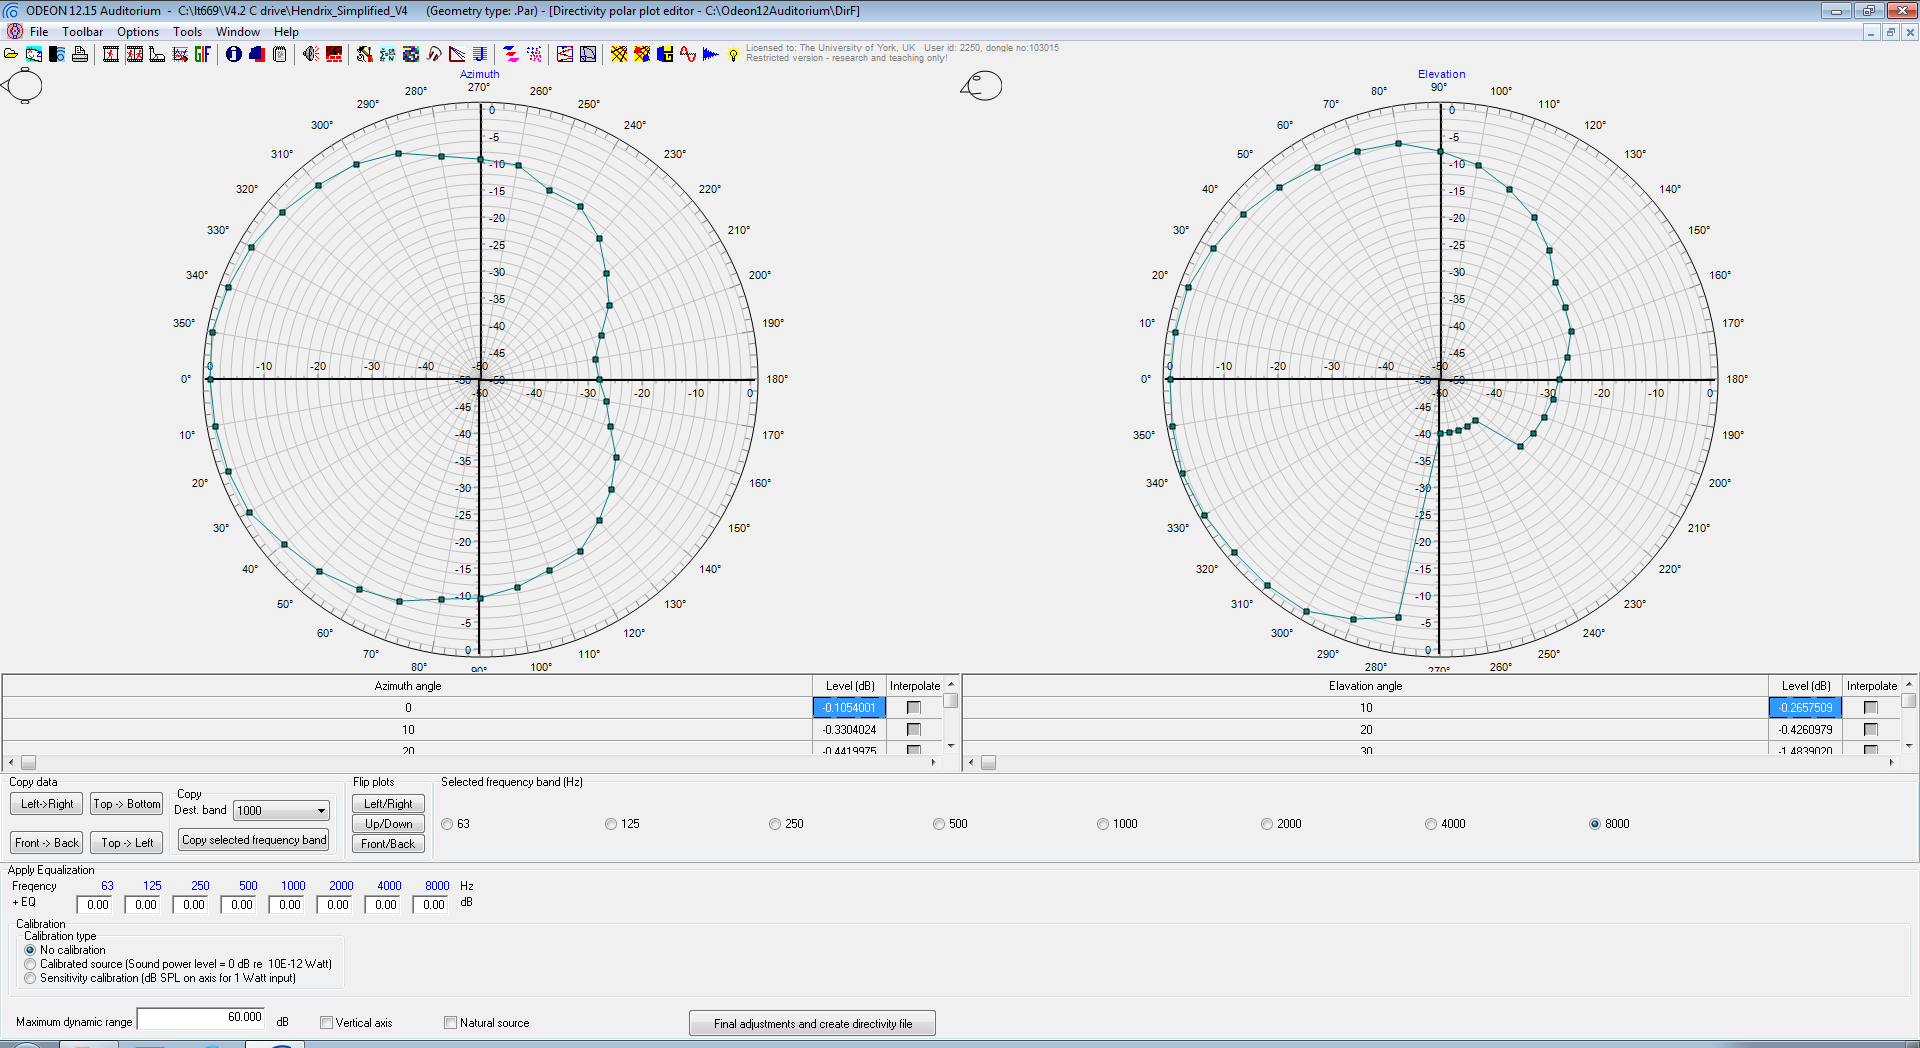
\includegraphics[scale = 0.3]{Sections/Implementation/Odeon/images/Directivity/DirectivityPattern.png}}
					\caption{Directivity pattern editor window in Odeon showing the directivity pattern for the horizontal plane (left) and the vertical plane (right) for the 8Khz octave band using data from \cite{calum}.}
					\label{directivity}
				\end{figure}


		\subsubsection{RIR Topology Problems}
		\label{odeonError}

			\paragraph{RIR Analysis}
			%Show original output RIR
			It has been noted that the \ac{RIR}'s produced will attempt to accurately resemble a human head. This involves placing the sound source below the receiver, to resemble the mouth (sound source) below the ears (receiver). When taking real \ac{RIR} measurements it is often not possible to get the source and receiver close enough due to the physical dimensions of the equipment used and therefore result in an unnatural distance between them (see section~\nameref{realRIRs}). However, with using software such as Odeon, where sound sources are calculated from a point source, it is possible to move the source and receiver much closer together. Initially, the sound source was placed 1m off the ground and the receiver was positioned 0.05m above the sound source. Three \ac{RIR}'s positioned along the centre of the room at varying distances from the left wall can be seen in figure~\ref{incorrectRIR}. (These \ac{RIR}'s are taken from grid positions 76, 77 and 83 respectively which can be seen in figure~\ref{bulkRIRs} and is explained in section~\nameref{rirlocations})

			


			%-------------Incorrect RIRs image-------------%
			\begin{figure}[H]
				\centerline{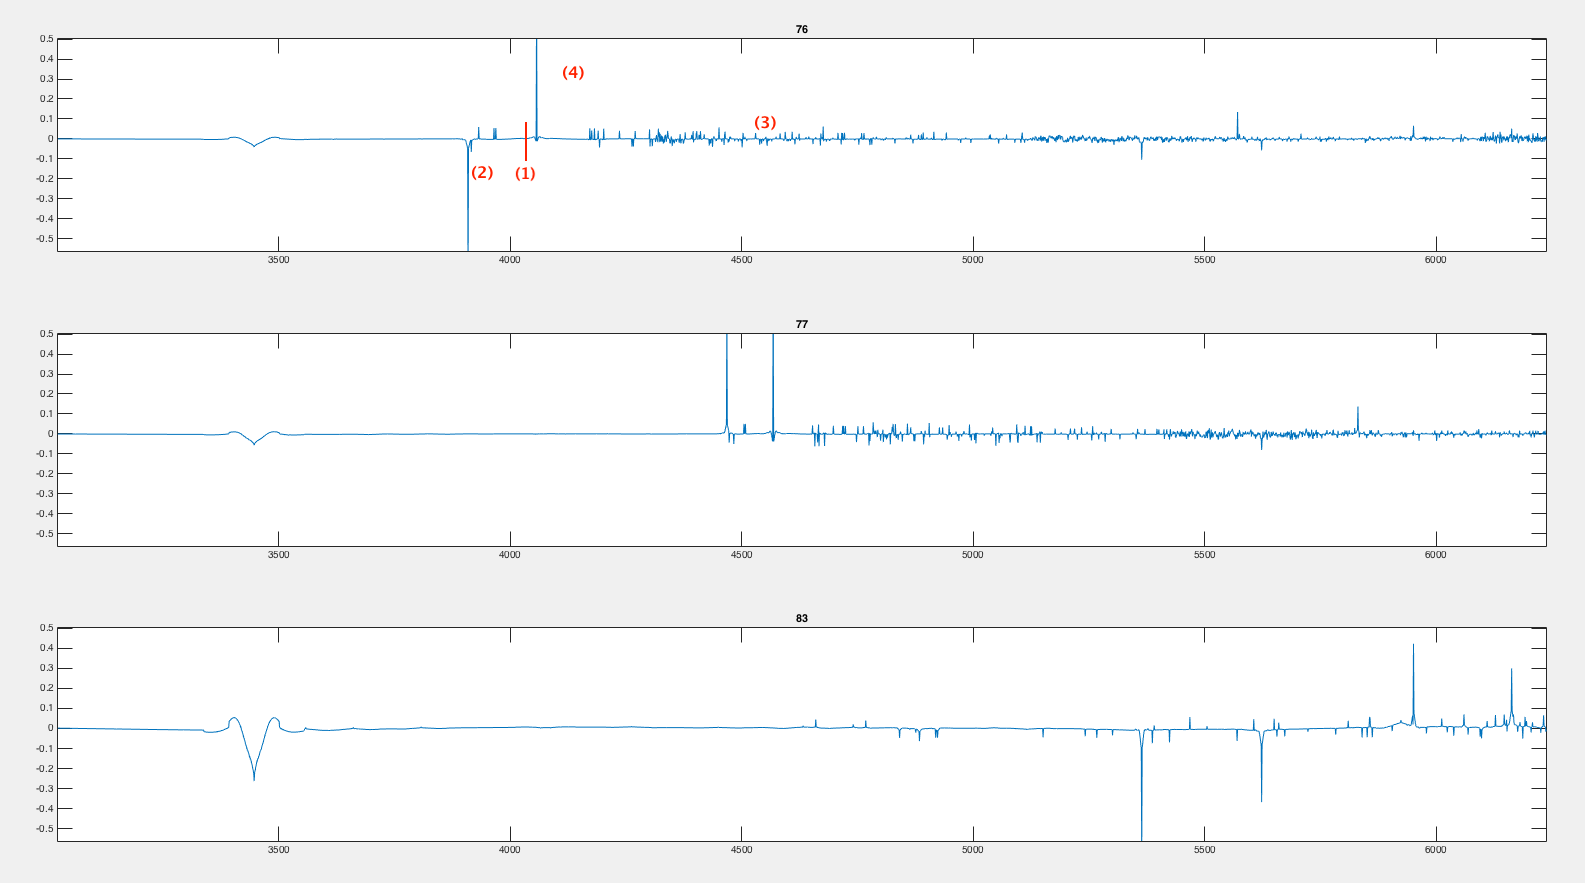
\includegraphics[scale = 0.33]{Sections/Implementation/Odeon/images/incorrectRIR/RIR_76_incorrect_edit.png}}
				\caption{Initial \ac{RIR} output with receiver 5cm above sound source showing \ac{RIR}'s from grid positions 76, 77 and 83 shown in figure~\ref{bulkRIRs}}
				\label{incorrectRIR}
			\end{figure}

			%-------------76 incorrect RIR image-------------%
			\begin{figure}[H]
				\centerline{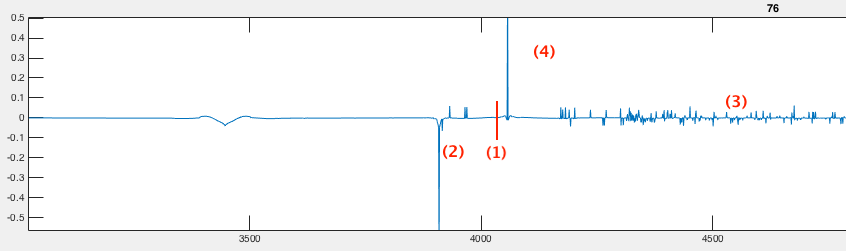
\includegraphics[scale = 0.5]{Sections/Implementation/Odeon/images/incorrectRIR/RIR_76_incorrect_edit_crop.png}}
				\caption{Initial \ac{RIR} output with receiver 5cm above sound source from grid position 76}
				\label{incorrectRIR_76}
			\end{figure}

			These \ac{RIR} positions were chosen as the varying distance from the left wall can be used to estimate when to expect reflection other than that from the floor which will remain the same across each \ac{RIR}. At the beginning of each plot, a dip of varying amplitude at the same instance in time can be seen. Without further inspection, this could be assumed as the direct sound from the source to receiver, which would be in the same place in time, as the source and receiver are kept the same distance across all RIRs, though the varying amplitude is questionable.

			Figure~\ref{incorrectRIR_76} shows the first \ac{RIR} from figure~\ref{incorrectRIR} which is used for the analysis of early reflections. The \ac{RIR}'s can be validated by calculating where expected reflections should be, using the following equation:
			
			\begin{equation}\label{distance}
				t_s = t_p - \frac{d}{c}
			\end{equation}
			where:

			\begin{tabular}{l l}
			$t_s$ & = Expected start of impulse (seconds)\\
			$t_p$ & = Time of first recorded reflection (first peak) (seconds)\\
			$d$ & = Distance between source and receiver (meters)\\
			$c$ & = Speed of sound ($344m/s$) \\
			\end{tabular}


			Therefore, if this dip is assumed to be the direct sound which occurs at $t_p = 0.03448s$ , where $d = 0.05m$, then the start of the impulse can be calculated to be:

			\begin{equation}
			 0.03448s - \frac{0.05m}{344m/s} = 0.03433s = t_s
			\end{equation}

			This is indistinguishable from the direct sound peak, which is understandable given the source and receiver are only separated by 0.05m. Now the expected start of this impulse is known, the expected first reflection due to the floor can be calculated:

			\begin{equation}
			\frac{2.05m}{344m/s} + t_s = 0.4029s
			\end{equation}

			However, it can be seen that the first reflection occurs at (2), at a time of $0.039s$ suggesting that sound has travelled 1.6392m before reaching the receiver. 

			\begin{equation}
			(0.039s - t_s)*c = 1.6382m
			\end{equation}

			However, the shortest available distance a sound could travel other than directly from the source to the receiver is 2.05m (the first floor reflection).

			As the source and receiver are placed 1.85m away from the left side wall (meaning sound has to travel slightly over twice this distance), a second reflection would be expected to occur at:

			\begin{equation}
			\frac{1.85m\times{2}}{c} + t_s = 0.04509s
			\end{equation}

			indicated by (3) in figure~\ref{incorrectRIR_76}. However, it can be seen that no strong reflection occurs here.

			After an email was sent to the technical department at Odeon \cite{odeonEmail}, it was suggested that the small dip at the beginging of the \ac{RIR} may be a bug in the version of Odeon being used. It could therefore be assumed that the direct sound is actually captured at the peak shown at (2) in figure~\ref{incorrectRIR_76} at a time of $0.03908$. From this the new expected time for the start of the impulse could be calculated:

			\begin{equation}
			0.03908s - \frac{d}{c} = 0.03893s = t_s
			\end{equation}

			It could then be assumed that the first reflection caused by the floor is the peak at (4) in figure~\ref{incorrectRIR_76} which occurs at a time of 0.04058s. However, this would suggest that sound has travelled 0.05532m:

			\begin{equation}
			(0.04058s - t_s)\times{c} = 0.05532m
			\end{equation}

			meaning that it has reflected off a surface approximately 0.28m away, of which there is no surface.

			It is also apparent that if the first peak other than the dip at the beginning of the file is taken to be the direct sound, it can be seen across the \ac{RIR} plots shown in figure~\ref{incorrectRIR} that these would occur at different times depending on room position. This is also incorrect as it has been mentioned that the source and receiver distance is kept constant for all \ac{RIR} simulations. The first strong reflection appears to be delayed in time the further away from the left side wall the RIRs are taken which would be accurate, however the timings are incorrect.

			\paragraph{Experiment}
			%Show Height Test Images
			After some further investigation, it was found that the Odeon Manual \cite{odeonManual} states in the section \textbf{Minimum distance from receiver to closest surface}:

			 \vspace{5mm}
			 \begin{center}
			 \begin{minipage}{0.75\textwidth}
			 ``\textit{If a receiver is placed very close to a surface then results will be sensitive to the actual position of the secondary sources generated by ODEON’s late ray method. If such a secondary source happens to be very close to the receiver, e.g. 1 to 10 centimetres, this may produce a spurious spike on the decay curve, resulting in unreliable predictions of the reverberation time [...] to avoid this problem it is recommended that distances to surfaces are kept greater than say 0.3 and 0.5 meters}''
			 \end{minipage}
			 \end{center}
			 \vspace{5mm}

			 Though this is a problem said to be caused by secondary sources, it can be assumed that this issue could also be caused by primary sources. This was investigated by producing \ac{RIR}'s with the source in a stationary location with receivers varying in distance above the source. Figure~\ref{HeightTest} shows six \ac{RIR}'s produced using different distances between the source and receiver where the numbers 1 - 6 indicate the following:

			 \begin{center}
				 \begin{tabular}{|c |c| c|}
				 \hline
				 \multirow{2}{*}{Graph Number} & \multicolumn{2}{|c|}{Distance from floor} \\ \cline{2-3}
				 & Source & Receiver \\\hline
				 (1) & 1m & 1.05m \\
				 (2) & 1m & 1.15m \\
				 (3) & 1m & 1.30m \\
				 (4) & 1m & 1.50m \\
				 (5) & 1m & 1.60m \\
				 (6) & 1m & 1.70m \\ \hline
				 \end{tabular}
			 \end{center}
			 \vspace{5mm}
		 	%-------------Height Test image-------------%
			\begin{figure}[h]
				\centerline{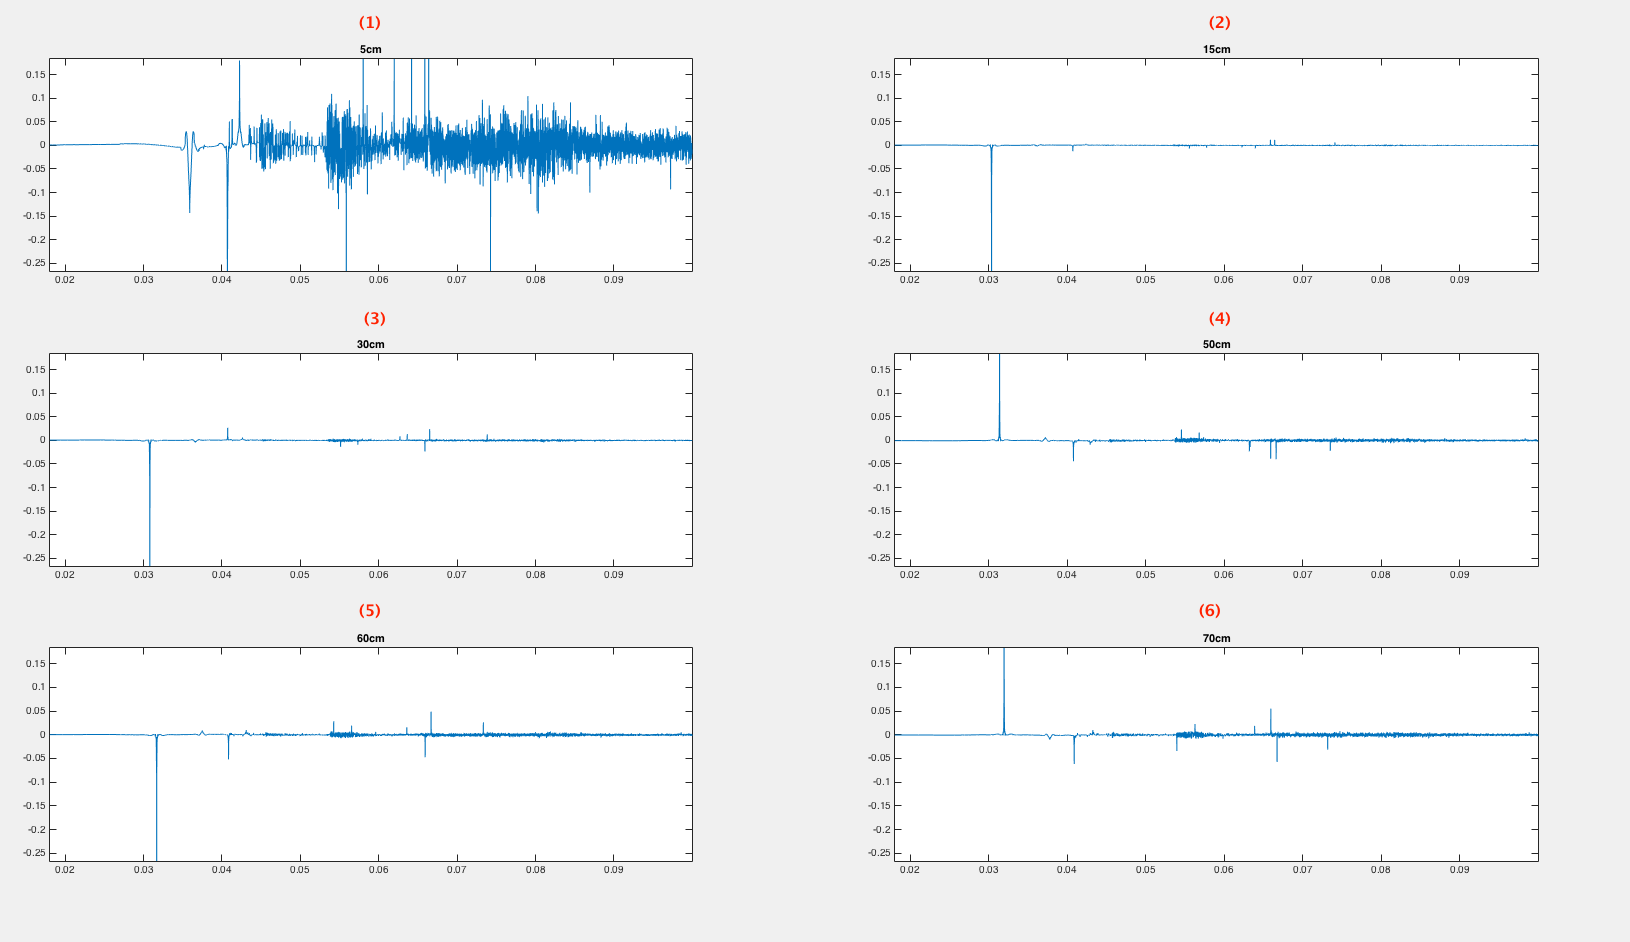
\includegraphics[scale = 0.32]{Sections/Implementation/Odeon/images/incorrectRIR/HeightTest_Edit.png}}
				\caption{Plots of \ac{RIR}'s produced with the receiver placed at varying distances from the source, indicated by the title of each plot where \textbf{(1)}: 5cm \textbf{(2)}: 15cm \textbf{(3)}: 30cm \textbf{(4)}: 50cm \textbf{(5)}: 60cm \textbf{(6)}: 70cm}
				\label{HeightTest}
			\end{figure}

			The following numbers (1) - (6) refer to the individual plots in figure~\ref{HeightTest}.

			A 5cm distance between the source and receiver shown in (1) was originally used. This plot can be seen to be greatly different from the rest (\textit{\textbf{Note:} The reason the \ac{RIR} shown in (1) looks different to previously investigated \ac{RIR}'s such as those in figure~\ref{incorrectRIR} is due to the plot being zoomed in, causing it to look greater in amplitude. This was done so it could be compared to (2) - (6) whilst being on the same scale}). It is in this \ac{RIR} that the `dip' found in the previously investigated \ac{RIR}'s is contained, whereas the \ac{RIR}'s with a greater distance between source and receiver (2) - (6) do not.

			\paragraph{Results}
			\label{odeon:results}
			%Show new RIRs with correct timings

			It is suggested in the Odeon manual (quoted above) that source and receiver be at least between 30cm and 50cm apart. Though a distance of 15cm (2) shows an \ac{RIR} similar to the rest of the assumed correct ones, it is obvious that there is one strong direct sound but it is difficult to see the other expected direct reflections, whereas when the receiver is moved further away from the source to a distance suggested by the Odeon manual, the early reflections become more obvious, with clarity of strong peaks being more consistent through (4) - (6). The peaks in the \ac{RIR} (5) (60cm) were investigated to assure their correctness, shown in figure~\ref{60cm}. This \ac{RIR} was chosen as the distance between the source and receiver for the real \ac{RIR}’s taken in Hendrix Hall was also 60cm. As the aim of achieving a more accurate human head topology was not possible due to this issue caused by Odeon, it was decided that for now, consistency is the next best thing.


						%-------------60cm image-------------%
			\begin{figure}[h]
				\centerline{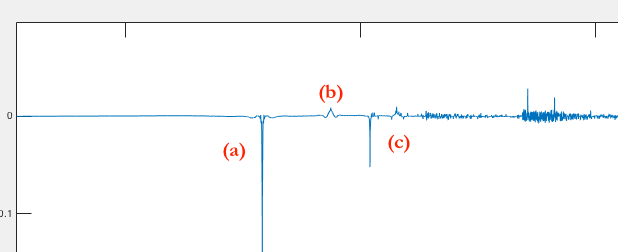
\includegraphics[scale = 0.6]{Sections/Implementation/Odeon/images/incorrectRIR/76_60cm_editV2_crop.png}}
				\caption{\ac{RIR} produced when the receiver is placed 60cm above the source.}
				\label{60cm}
			\end{figure}


			The first peak (a) can be assumed to be the direct sound, present at $0.03168s$, meaning the start of the impulse can be calculated using equation~\ref{distance}, where $d = 0.6$:

			\begin{equation}
			0.03168s - \frac{0.6m}{c} = 0.02994s = t_s
			\end{equation}

			From this, it can be calculated that the peak at (b), which occurs at $0.0375s$ had been captured after sound has travelled 2.6m:

			\begin{equation}
			(0.0375s - t_s)\times{c} = 2.6m
			\end{equation}

			This is the reflection from the floor which is 1.6m below the receiver, causing the sound to travel 1m to the floor and then a further 1.6m to reach the receiver. This is shown in \textbf{Path 1} in figure~\ref{reflectionPaths}. The peak at (c), occurring at $0.04084s$ can be calculated as having travelled 3.74m which is the distance travelled by a reflection caused by the left side wall shown as \textbf{Path 2} in figure~\ref{reflectionPaths}.

				%-------------reflection path image-------------%
			\begin{figure}[H]
			\centerline{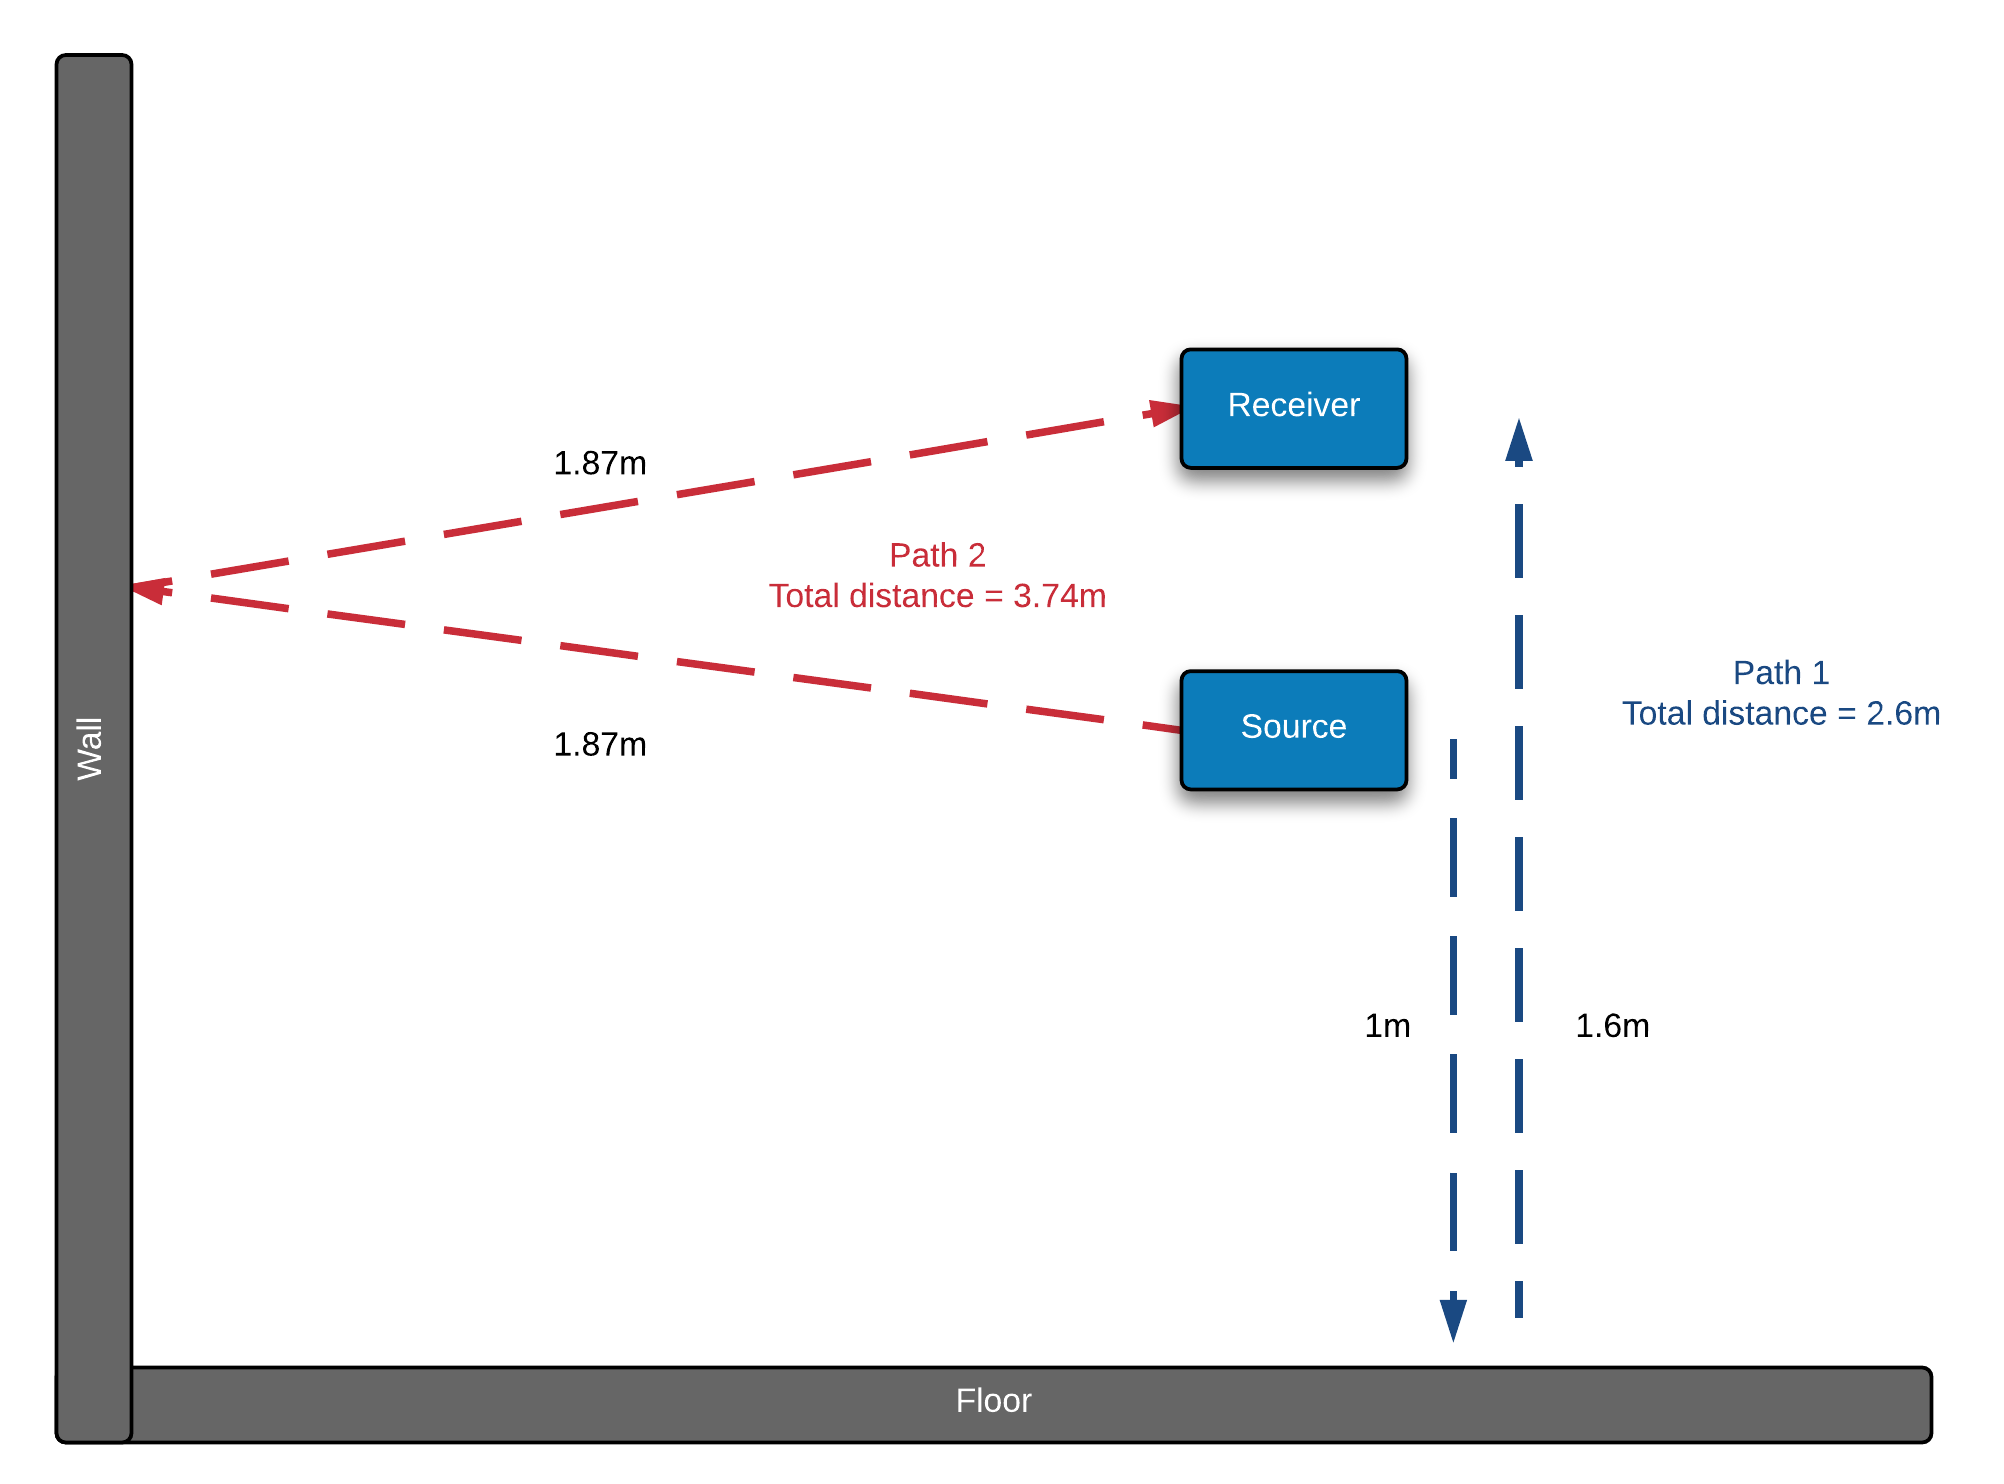
\includegraphics[scale = 0.25]{Sections/Implementation/Odeon/images/incorrectRIR/reflectionPaths_colourV2.png}}
				\caption{Illustration of the two early reflection paths due to the floor and left side wall when the receiver is placed 60cm above the source.}
				\label{reflectionPaths}
			\end{figure}

			It can therefore be stated that the \ac{RIR}'s with a distance of 60cm between the source and receiver are accurate and can be used to produce a mass of \ac{RIR}'s.

		\subsubsection{RIR Locations}
		\label{rirlocations}
			%How many RIRs and where?
			As discussed in section~\nameref{Background:RIRPositions}, \ac{RIR}'s were to be taken every 1m starting from the centre of the room and form a grid (rectangular or square). However, there were some positions within the room that would cause some \ac{RIR} positions to be invalid. The location of these invalid positions could be found anywhere the sound source and receiver were placed closer than 0.75m to a surface. As the distance between the centre of the \ac{VSS} (where the listener would be located) and the surrounding loudspeakers is approximately 1.5m, it would be impossible to reproduce a sound that has to travel less than this distance in the virtual space at the correct time, thus direct reflection from surfaces closer than 0.75m cannot be reproduced in time. When taking this into account, figure~\ref{incorrectRIRPositions} shows the positions that would be invalid due to them being placed too close to a surface, marked as U, V, W and Z. W represents a large space of invalid \ac{RIR} positions and they would all be too close to the table surfaces.

			%-------------RIR Invalid Positions Image-------------%
			\begin{figure}[H]
				\centerline{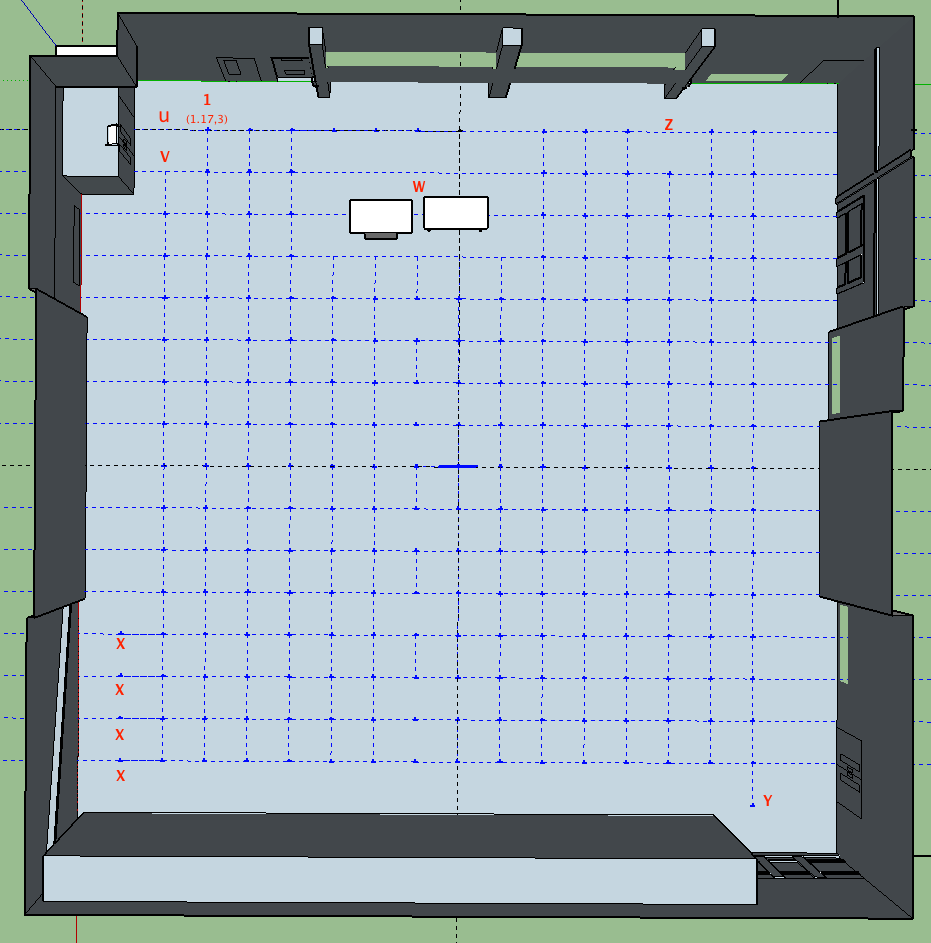
\includegraphics[scale = 0.37]{Sections/Implementation/Odeon/images/RIRPositions/RIRPositionAnnotated.png}}
				\caption{Top down view of the Hendrix Hall model indicating the \ac{RIR} positions that are invalid due to being too close to a surface (U, V, W and Z), where other \ac{RIR}'s that are valid are not included as it would cause inconsistency (X and Y)}
				\label{incorrectRIRPositions}
			\end{figure}

			It was decided however that these \ac{RIR}'s would still be produced and used as part of the final system. If they were not included, there would be large gaps in the space where the user would have to jump between, thus be unable to produce what would feel like a consistent path.

			It was also later discovered (see section \nameref{latency}) that the latency due to the software used would mean that the beginning of the \ac{RIR}'s would have to be trimmed anyway, avoiding this issue altogether.

			There are several \ac{RIR}'s in figure~\ref{incorrectRIRPositions} labeled X and Y. These positions would still produce valid \ac{RIR}'s, however they were not included in the final grid as they would cause inconsistencies in the positions available to the user. All other blue crosses in figure~\ref{incorrectRIRPositions} were also included in the final \ac{RIR} grid, producing a grid 15x16, totalling 240 available positions. Figure~\ref{bulkRIRs} shows the final maximum available \ac{RIR}'s locations.

				%-------------RIR Invalid Positions Image-------------%
			\begin{figure}[H]
				\centerline{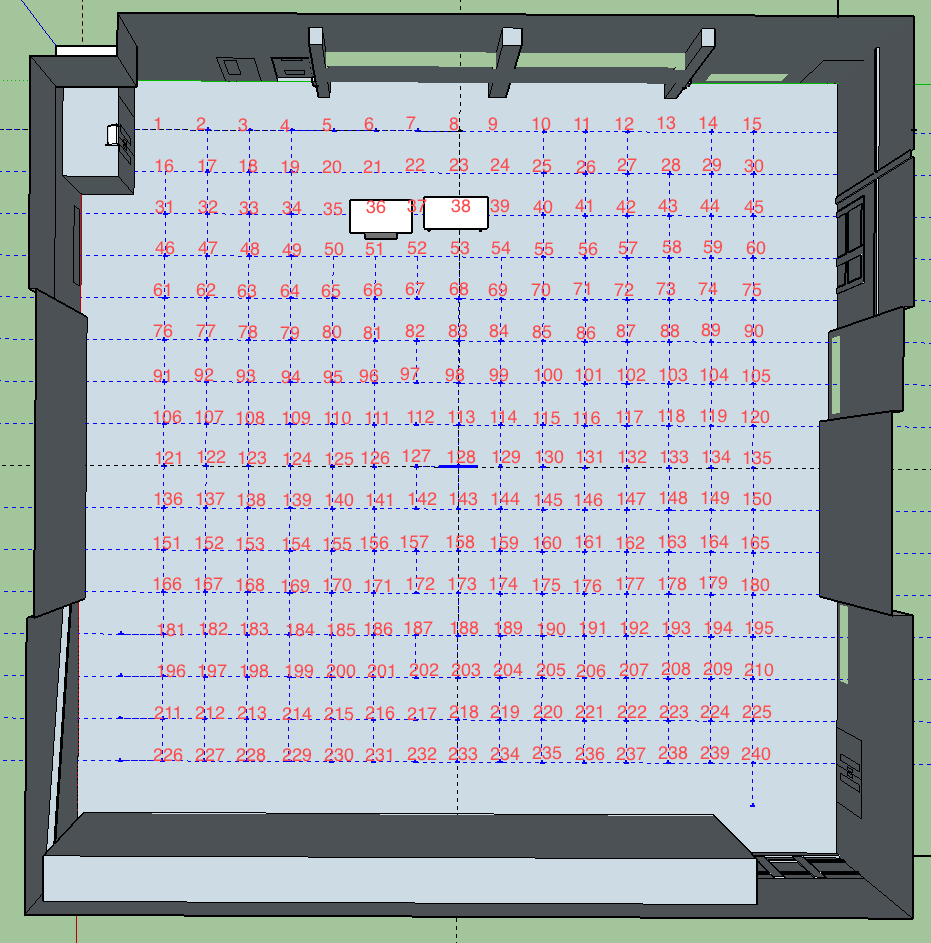
\includegraphics[scale = 0.37]{Sections/Implementation/Odeon/images/RIRPositions/RIR_Position_Bulk.png}}
				\caption{Top down view of the Hendrix Hall model showing the maximum number available \ac{RIR} locations.}
				\label{bulkRIRs}
			\end{figure}

		\subsubsection{RIR Rendering}
			\label{odeon:rendering}

			The source and receiver positions can be set using a .SouRecScript file, which contains information regarding the Cartesian coordinates of both sources and receivers within the room as well as the sound source directivity pattern and the direction in which the source is facing (available \href{file:///Users/Lewis%201/Uni%20Work/4th%20Year/Project/Write%20Up/Web%20Page/lt669.github.io/pages/Bulk_0.SouRecScript}{here} or file 4.2.2). This made rendering 240 \ac{RIR}'s almost effortless. However, once the script had set the locations of the source and receivers, each source and receiver had to be paired up individually. This is because Odeon provides a \textbf{Job List}, where any number of \ac{RIR}'s can be rendered one after another automatically, allowing the process to run without user interaction. For this to work, the user must tell Odeon which receiver to use for each sound source. Figure~\ref{SouRecPos} shows the job list menu where each source has to be connected to each receiver, using a series of drop down menus and scroll bars. This part of Odeon is clumsy and in no way designed to make the process fast and simple. This had to be done for all 240 \ac{RIR}'s and then again for the other three sets of \ac{RIR}'s used for facing different directions within the room, totalling 960 \ac{RIR}'s.

			%-------------RIR Invalid Positions Image-------------%
			\begin{figure}[H]
				\centerline{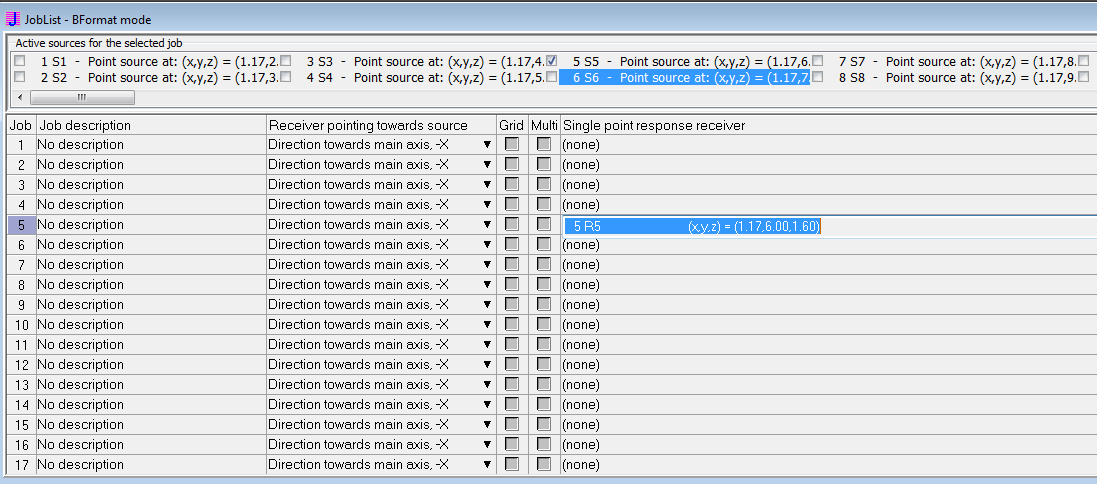
\includegraphics[scale = 0.54]{Sections/Implementation/Odeon/images/SouRecPos/SouRecSelection_crop.png}}
				\caption{Source and receiver pairing window in Odeon}
				\label{SouRecPos}
			\end{figure}

			A naming system was used for the \ac{RIR} files to indicate which grid positions they were taken from and which direction they were facing. For example: `008\_0.wav' is an \ac{RIR} from grid position 8 with 0\textdegree~rotation (facing the front of the room) where `128\_90' is taken from grid position 128 and has a 90\textdegree~rotation (facing the left side wall).

	\subsection{Producing Different RIR Grids}
	\label{odeon:grids}
		As described in section~\nameref{Background:RIRPositions}, user test \#3 requires there to be a number of available \ac{RIR} grids to choose from, each containing \ac{RIR} locations separated by a fixed distance. It was decided that there would be a total of 5 grids to choose from, the first (the one already produced) containing \ac{RIR}'s separated by 1m, the second grid containing \ac{RIR}'s separated by 2m and so on.	 Four Matlab algorithms were written (fully commented code available: \href{http://lt669.github.io/code/matlab/html/renameSortFiles.html}{renameSortFiles.m}) to extract the appropriate \ac{RIR}'s required for each new gird, and rename them starting from 001 up to the maximum number of \ac{RIR}'s in each grid. This made it easily integrable with the software described in section~\nameref{software}.

		The four grids can be seen in figures~\ref{2m},~\ref{3m},~\ref{4m} and~\ref{5m} respectively in~\nameref{appendixB}, showing which \ac{RIR} locations from the original grid they contain. The \ac{RIR} files for all 5 grids can be found in file 3.2


	\subsection{RIR Calibration}
		
		As both sets of \ac{RIR}'s that were to be used for user test \#1 were produced using different methods, it was imperative that they were calibrated to prevent the difference in level from influencing the participants perception of movement. As the real \ac{RIR}'s were louder than the synthetic ones and the fact that there were far fewer real \ac{RIR} measurements than synthetic ones, the real measurements were reduced in level to match those produced by Odeon.

		\subsubsection{Matlab}

			\paragraph{Method}
			% In an attempt to perfectly reduce the level of the real \ac{RIR}'s to match those of the synthetic ones, using Matlab, a multiplier was calculated by taking the RMS level of each of the 4 channels (W,X,Y,Z) in both the real and synthetic \ac{RIR}'s (illustrated using the following pseudo code):

			In an attempt to perfectly reduce the level of the real \ac{RIR}'s to match those of the synthetic ones, using Matlab, a multiplier was calculated by taking the RMS level of both the real and synthetic \ac{RIR}'s (illustrated using the following pseudo code):

			\vspace{3mm}
			\begin{center}
				\texttt{multiplier = RMS(real)/RMS(synthetic)}\\
				% \texttt{X channel multiplier = RMS(real Y channel)/RMS(synthetic X channel)}\\
				% \texttt{Y channel multiplier = RMS(real X channel)/RMS(synthetic Y channel)}\\
				% \texttt{Z channel multiplier = RMS(real Z channel)/RMS(synthetic Z channel)}\\
			\end{center}
			\vspace{3mm}

			This value was used to multiply each of the samples in the real \ac{RIR} to reduce each of the levels to that of the synthetic \ac{RIR}. The full matlab script used can be \href{http://lt669.github.io/code/matlab/html/calibrateAll.html}{calibrateALL.m} can be viewed or found in file 2.

			Figure~\ref{calRMS} shows the plots of both of the original \ac{RIR}'s (top = real, centre = Odeon) and the calibrated version of the real \ac{RIR} (bottom). As it can be seen, the peaks of the calibrated real \ac{RIR} fall within the same range as the synthetic \ac{RIR} (-0.02 to 0.02). However, when these \ac{RIR}'s were convolved with an audio sample taken from OpenAir \cite{singingSample} (available \href{http://lt669.github.io/pages/audioSamples.html}{here} or file 1.1 as \texttt{Singing.wav}), it still sounded significantly louder than that of the synthetic RIR convolved with the same audio sample.

			This can be heard in audio examples: \texttt{calRMSConv.wav} (calibrated real \ac{RIR}) and \texttt{odeonConv.wav} (Odeon \ac{RIR}) found \href{http://lt669.github.io/pages/audioSamples.html}{here} or in file 1.2

			%-------------RMS calibrated RIR Image-------------%
			\begin{figure}[H]
				\begin{center}
					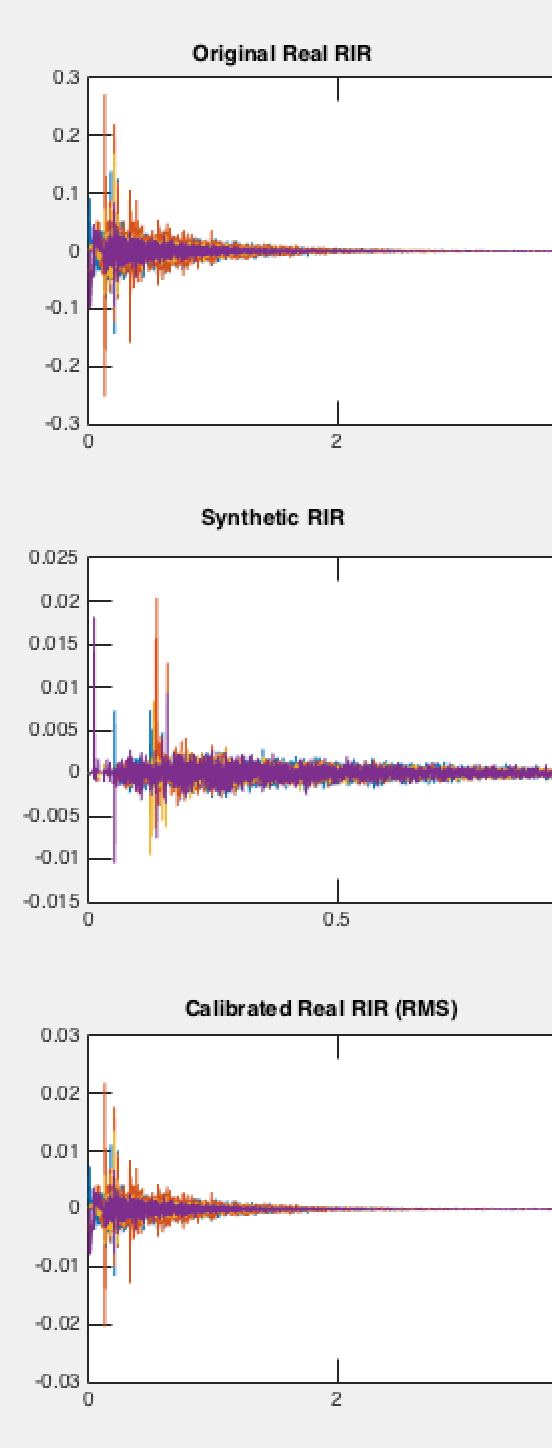
\includegraphics[scale = 0.3]{Sections/Implementation/RealRIRs/images/calibration/CalRMS_RIR_edit2.png} 
					\caption{Plots of the original real \ac{RIR} (top), the synthetic \ac{RIR} (centre) and the calibrated real \ac{RIR} (bottom) using the multiplier calculated using the RMS ratio value, showing that the peaks of the calibrated \ac{RIR} sit approximately within the same range as the synthetic \ac{RIR} (-0.02 to 0.02). (All 4 channels for each \ac{RIR} are shown as they will not all sit within the same amplitude limits, hence the different coloured waves in each plot).}
					\label{calRMS}
				\end{center}
			\end{figure}

			As can be seen in figure~\ref{calRMSsing}, the amplitude of the peaks in the signal convolved with the calibrated RIR are just over double those in the synthetic RIR convolved with the sample thus is perceived as louder.

			%-------------RMS calibrated Convolved Image-------------%
			\begin{figure}[H]
				\begin{center}
					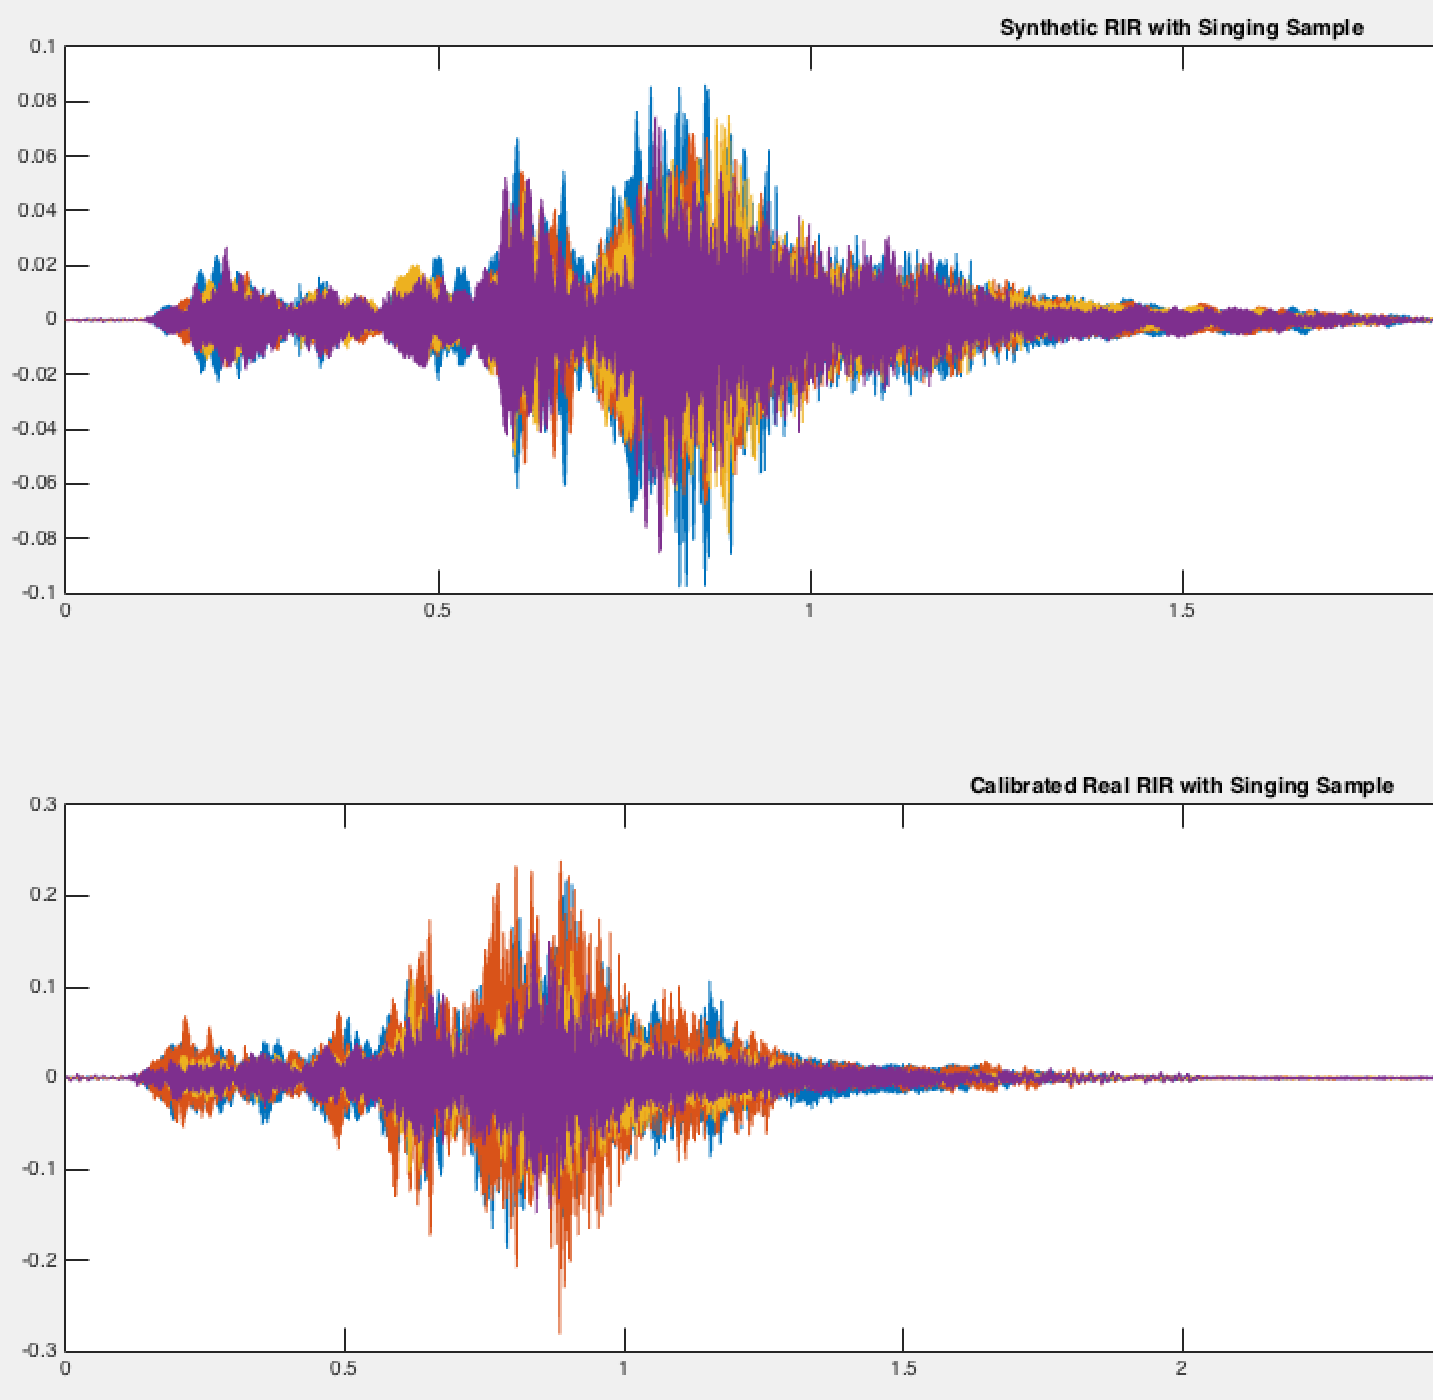
\includegraphics[scale = 0.3]{Sections/Implementation/RealRIRs/images/calibration/CalRMS_Sing_edit.png} 
					\caption{Plots of the synthetic \ac{RIR} (top) and the RMS calibrated real \ac{RIR} (bottom) convolved with an anechoic audio sample showing that the peaks of the calibrated \ac{RIR} convolved sample sit approximately in the range double that of the synthetic \ac{RIR} convolved sample, thus is perceived as louder.}
					\label{calRMSsing}
				\end{center}
			\end{figure}

			% Several manual values for the multiplier were tried instead, starting from 0.7 down to 0.2. It was found that a value of 0.3 normalized the real \ac{RIR}'s to the desired level. Figure~\ref{calMan} shows that the level of the manually calibrated RIR falls within a range of values half the magnitude of those found in the synthetic RIR. As magnitude of the RMS calibrated audio sample sits within a range of value twice as large as the synthetic \ac{RIR} sample, now that the peaks of the manually calibrated \ac{RIR} sit within half the synthetic \ac{RIR}'s range, it makes sense that the audio samples now approximately lay within the same range, as can be seen in figure~\ref{calMansing}.

			Several manual values for the multiplier were tried instead, starting from 0.7 down to 0.2. It was found that a value of 0.3 normalized the real \ac{RIR}'s to the desired level. Figure~\ref{calMan} shows that the level of the manually calibrated RIR falls within a range of values half the magnitude of those found in the synthetic RIR, which then makes the magnitude of the manually calibrated audio sample (shown in the bottom of figure~\ref{calMansing}) approximately the same level as the audio file produced using the synthetic \ac{RIR}.			

					%-------------Manually calibrated RIR Image-------------%
			\begin{figure}[H]
				\begin{center}
					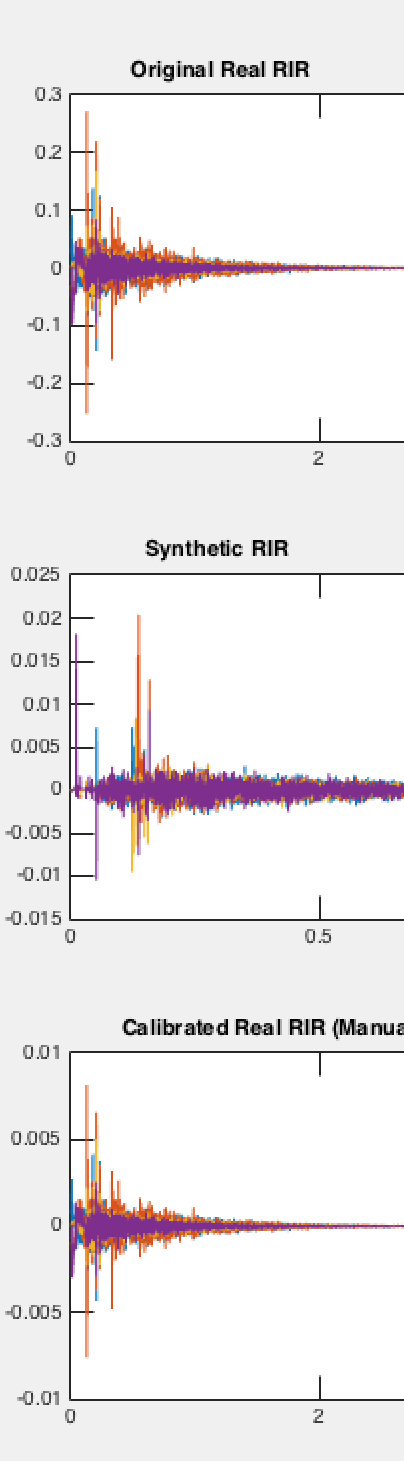
\includegraphics[scale = 0.3]{Sections/Implementation/RealRIRs/images/calibration/CalMan_RIR_edit.png} 
					\caption{Plots of the original real \ac{RIR} (top), the synthetic \ac{RIR} (centre) and the \textit{manually} calibrated real \ac{RIR} (bottom) showing that the peaks of the manually calibrated \ac{RIR} sit within half of the range of the synthetic \ac{RIR}.}
					\label{calMan}
				\end{center}
			\end{figure}

			%-------------Manually Calibrated Convolved Image-------------%
			\begin{figure}[H]
				\begin{center}
					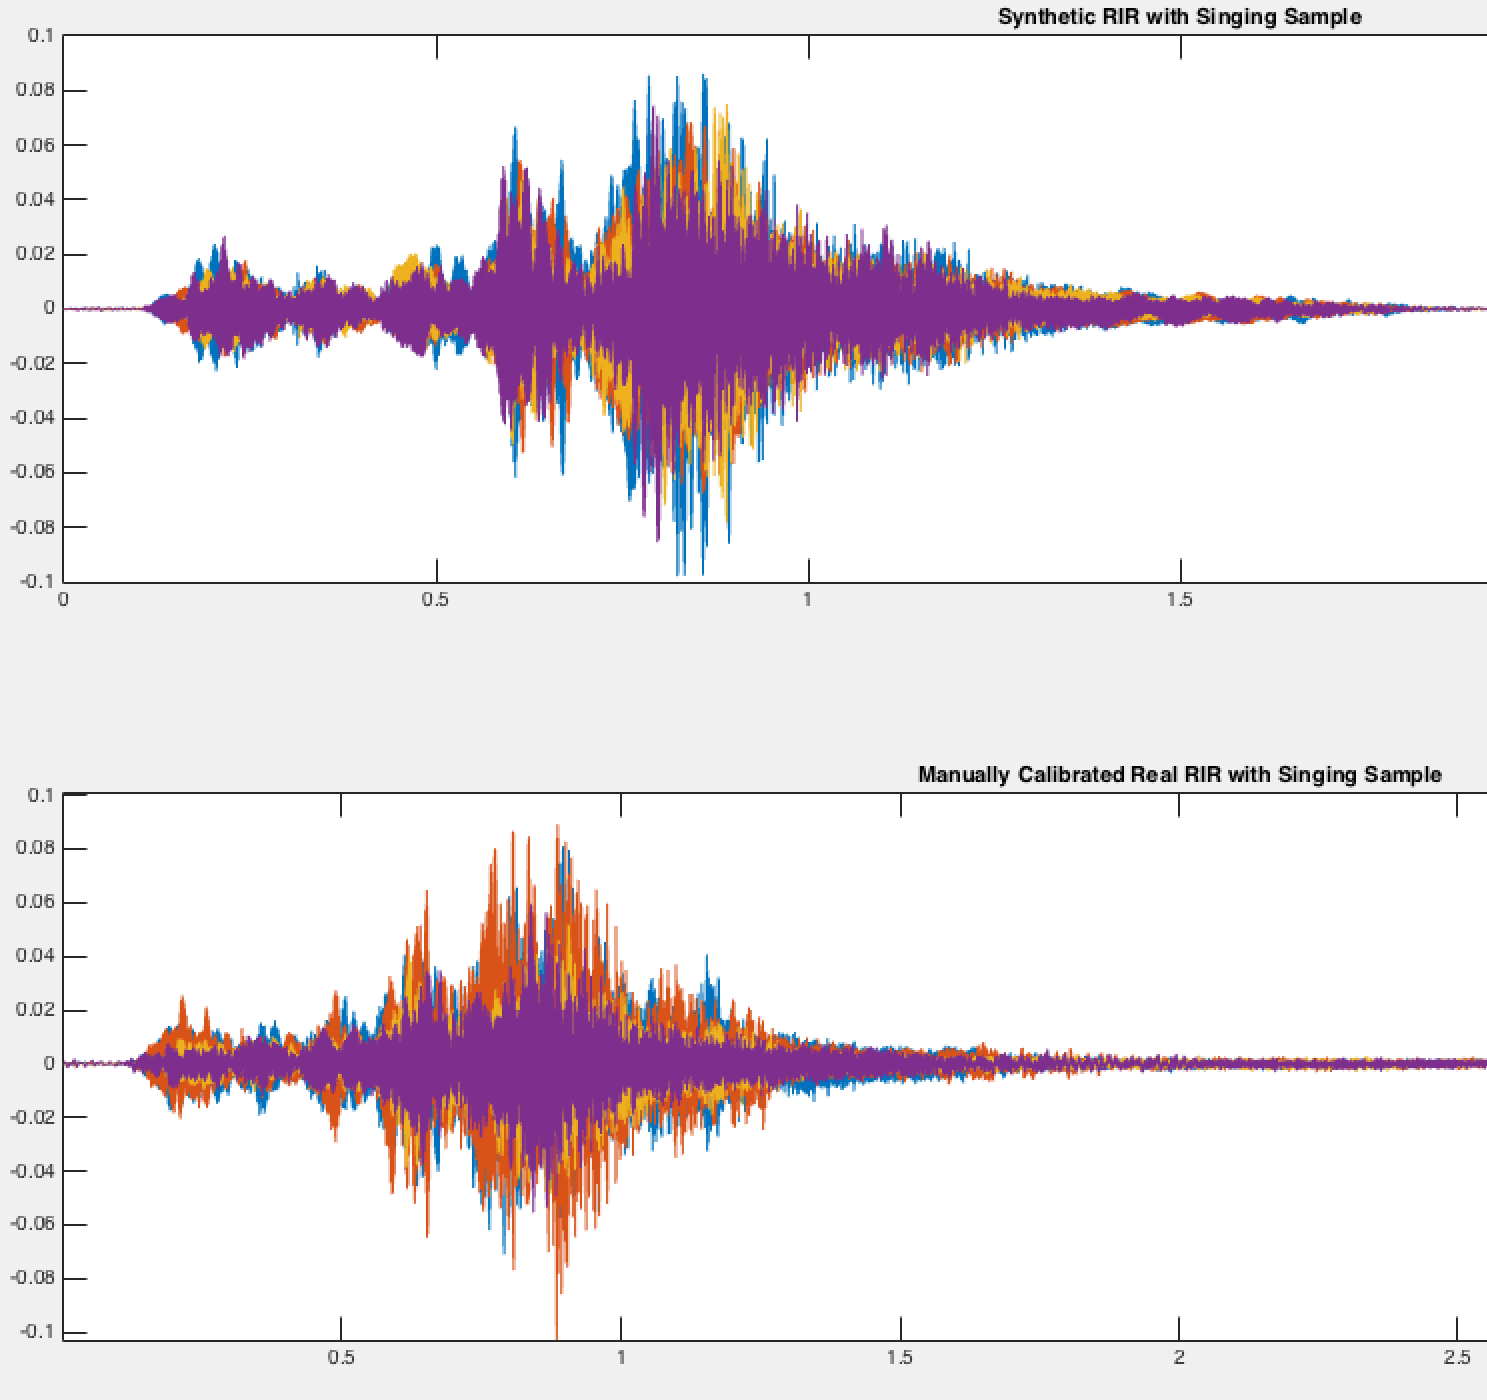
\includegraphics[scale = 0.3]{Sections/Implementation/RealRIRs/images/calibration/CalMan_Sing_edit.png} 
					\caption{Plots of the synthetic \ac{RIR} (top) and the RMS calibrated real \ac{RIR} (bottom) convolved with an anechoic audio sample showing that the speaks of the calibrated \ac{RIR} convolved sample sit approximately in the range double that of the synthetic \ac{RIR} convolved sample.}
					\label{calMansing}
				\end{center}
			\end{figure}

		\paragraph{Issue}
			After listening to the convolved audio file more closely, it could be heard that the tail of the reverb seemed to increase in volume, producing what sounded like a `swelling' effect. Figure~\ref{pulse} shows the reverb tail of the manually calibrated convolved audio sample, where small pulses (occurring approximately every 0.05s), thought to be the culprit of this undesired trait, can be seen (mostly in the channel shown in yellow). Further investigation did not reveal the cause of the pulsing. The effect of the pulse can be heard in the audio sample pulseExample.wav found \href{http://lt669.github.io/pages/audioSamples.html}{here} or in file 1.2.

			%-------------Pulse Image-------------%
			\begin{figure}[H]
				\begin{center}
					\includegraphics[scale = 1]{Sections/Implementation/RealRIRs/images/calibration/cal_pulse.png} 
					\caption{Reverb tail of the audio sample convolved with the manually calibrated \ac{RIR} showing a pulse like pattern.}
					\label{pulse}
				\end{center}
			\end{figure}

			As the cause of the problem could not be uncovered within the time allocated, a less accurate but plausible manual calibration method was used.

		\subsubsection{Reaper}

			All of the real \ac{RIR} files were imported into Reaper and send through a bus to a master channel in order to normalise all \ac{RIR}'s evenly. These were then compared by ear to a synthetic \ac{RIR} and manually level matched. The closest match was by reducing the level of the real \ac{RIR}'s by 28.6dB. Though this method is less accurate, it prevented any unwanted errors in the signal such as those caused by using Matlab and allowed for the job to be done within a reasonable amount of time.

		\subsection{Room Modelling and Synthetic RIR Rendering Summary}


			As stated in section \nameref{background:aims}, one benefit of using the direct \ac{RIR} rendering method is that it is simple. The process of obtaining the desired \ac{RIR}'s has shown that though time consuming, no complex procedures were undertaken.

			% The fact that this process was time consuming can be put down to two points:
			% \begin{enumerate}
			% 	\item Inexperience
			% 	\item Starting from scratch
			% \end{enumerate}

			% Though in this case, the dimensions of the building in question had to be obtained, it would be much faster to work from existing blueprints.


			%Adding directivity is a bonus
			A benefit of using Odeon to obtain these \ac{RIR}'s is that it has allowed for the directivity of a human head has been modelled, thus providing a more accurate sound source directivity pattern than would have otherwise been achieved and was no more hassle to do than rendering \ac{RIR}'s using Odeons standard omni-directional point source.
			
			%Still easier to produce bulk RIRs

			%Odeon room materials are lacking
			However, other aspects of the Odeon software effected the accuracy of the \ac{RIR} produced, such as the material list. Though the material list could be edited and built upon, the fact that its initial available options were limited instantly reduced the possibility for an accurate simulation of room acoustics. It has been shown that it is possible to achieve a close to desired result through the manipulation of the materials absorption coefficients, however this issue coupled with the already stated issues of geometrical acoustic modelling methods regarding their accuracy diminishes the plausibility of the system. In addition, the extra time spend on tweaking the resultant \ac{RIR}'s is not desirable, however this can be said for any modelling technique that involves simulation, thus is not restricted to this project alone.

			Though it has been shown that producing 960 \ac{RIR}'s can be done sat in front of a computer, Odeon is not optimised for such a task. As stated in \nameref{odeon:rendering}, though it is possible to import a simple script to set all of the source and receiver locations, having to join them up one at a time takes the best part of an hour of repetitive point, clicking and dragging and for this project has to be done four times over. This undesirable software flaw would be simply fixed by adding the option to pair them up within the source and receiver script. In addition to this, though the required distance between the source and receiver in order to prevent erroneous calculations is larger than desired, it is still possible to place them closer together than it is when using physical equipment to measure real \ac{RIR}'s. 
			
			In summary, a large grid of 960 \ac{RIR}'s in 240 locations within a virtual space of choosing have been relatively easily produced, providing a good approximation of its room acoustics. The only real issue faced was software that is not optimised for such a task.


	
\end{document}